\documentclass[9pt]{sigplanconf}
\usepackage{etex}
\usepackage{float}
\usepackage{mathrsfs}
\usepackage{booktabs}
\usepackage{boxedminipage}
\usepackage[T1]{fontenc}
\usepackage{epsfig}
\usepackage{multirow}
\usepackage{url}
\usepackage[normalem]{ulem}
\usepackage{schemepgm}
\usepackage{graphicx}
\usepackage{graphpap}
\usepackage{tabularx}
\usepackage{amssymb}
\usepackage{amsmath}
\usepackage{pstricks}
\usepackage{pst-text}
\usepackage{pst-node}
\usepackage{pst-tree}
\usepackage{pst-rel-points}
\usepackage{bcprules}
\usepackage{subfigure}
\usepackage[boxed]{algorithm2e}
\usepackage{makecell}

%%%%%%%%%% IMPERATIVE %%%%%%%%%%%%

%%%%%%%%%%%%%%%%%%%%%%%%%%%%%%%%%%%%%%%%%%%%%%%%%%%%%%%%%%%%%%%%%%
%%% Comment out a part of latex document
\newcommand{\cmt}[1]{}
\newcommand{\akadd}[1]{\protect{\red  #1}}
\newcommand{\akdel}[1]{\protect{\blue #1}}
\newcommand{\del}[1]{\protect{\magenta #1}}

\newcommand{\mybox}{\hfill\ensuremath{\Diamond}}
\newcommand{\NDIn}[1]{\mbox{\sf In$_#1$}}
\newcommand{\NDOut}[1]{\mbox{\sf Out$_#1$}}
%\newcommand{\x}{\cx}
%\newcommand{\y}{\cy}
%%%%%%%%%%%%%%%%%%%%%%%%%%%%%%%%%%%%%%%%%%%%%%%%%%%%%%%%%%%%%%%%%%

%%%%%%%%%%%%%%%%%%%%%%%%%%%%%%%%%%%%%%%%%%%%%%%%%%%%%%%%%%%%%%%%%%
%%%% Programs in latex 
\protect{\newlength{\FTABL}}
\protect{\newlength{\TABL}}
\protect{\newlength{\BRACE}}
\settowidth{\BRACE}{\{}

%%%%%%%%%%%%%%%%%%%%%%%%%%%%%%%%%%%%%%%%%%%%%%%%%%%%%%%%%%%%%%%%%%

 \newcommand{\ntbar}{\ensuremath{\overline\nt}}
%% %%%%%%%%%%%%%%%%%%%%%%%%%%%%%%%%%%%%%%%%%%%%%%%%%%%%%%%%%%%%%%%%%%
%%% Special pictures
\newcommand{\myarrow}{\mbox{%
 \psset{unit=1cm}%
 \begin{pspicture}(0,0)(.27,.2)%
  \psline[linewidth=.15mm]%
  (0,.1)(.125,.1)(.125,.035)(.25,.1)(.125,.165)(.125,.1)%
  \end{pspicture}}%
} 



%%
%% paths and derefs
\newcommand{\epath}{\mathsf{ep}}
\newcommand{\paths}{{\sf paths}}
\newcommand{\dpaths}{{\sf dpaths}}
\newcommand{\Pf}[2]{\ensuremath{\Pfonly_{\!\!#1}^{\,#2}}}
\newcommand{\Pfonly}{\ensuremath{\mathsf{PF}}}
\newcommand{\Pp}[2]{\ensuremath{\Pponly_{\!\!#1}^{\,#2}}}
\newcommand{\Pponly}{\ensuremath{\mathsf{PP}}}
\newcommand{\Pe}[3]{\ensuremath{\Peonly(#1, #2, #3)}}
\newcommand{\Peonly}{\ensuremath{\mathsf{PE}}}
\newcommand{\Peb}[3]{\ensuremath{\Pebonly(#1, #2, #3)}}
\newcommand{\Pebonly}{\ensuremath{\Peonly!}}
\newcommand{\Pv}{\ensuremath{\mathsf{P}}}
\newcommand{\Pvphi}{\ensuremath{\Pv^\emptyset}}
\newcommand{\Ddf}[2]{\ensuremath{\Ddfonly_{\!\!#1}^{\,#2}}}
\newcommand{\Ddfonly}{\ensuremath{\mathsf{DF}}}
\newcommand{\Dp}[2]{\ensuremath{\Dponly_{\!\!#1}^{\,#2}}}
\newcommand{\Dponly}{\ensuremath{\mathsf{DP}}}
\newcommand{\De}[3]{\ensuremath{\Deonly(#1, #2, #3)}}
\newcommand{\Deonly}{\ensuremath{\mathsf{DE}}}
%%\newcommand{\Deb}[3]{\ensuremath{\Debonly(#1, #2, #3)}}
%%\newcommand{\Debonly}{\ensuremath{\Deonly!}}
\newcommand{\Dv}{\ensuremath{\mathsf{D}}}
\newcommand{\Dvphi}{\ensuremath{\Dv^\emptyset}}
\newcommand{\derefs}{{\sf derefs}}

\newcommand{\bw}[1]{\ensuremath{\overline{#1}}} % backward
\newcommand{\cat}[2]{\ensuremath{#1#2}} % concat
\newcommand{\expshare}{\ensuremath{\mathsf{ExpS}}} % generic path

%% heap location and heap cell
\newcommand{\loc}[1]{\ensuremath{\mbox{\sf Loc}[{#1}]}}
\newcommand{\cell}[1]{\ensuremath{\mbox{\sf Cell}[{#1}]}}

%% type of labels
\newcommand{\acar}{\ensuremath{\mathbf{0}}}
\newcommand{\acdr}{\ensuremath{\mathbf{1}}}
\newcommand{\bcar}{\ensuremath{\bar\acar}}
\newcommand{\bcdr}{\ensuremath{\bar\acdr}}
\newcommand{\clazy}{\ensuremath{{\mathbf{2}}}}
\newcommand{\bX}  {\ensuremath{\bar{X}}}
\newcommand{\acarset}{\ensuremath{\lbrace\acar\rbrace}}
\newcommand{\acdrset}{\ensuremath{\lbrace\acdr\rbrace}}
\newcommand{\bcarset}{\ensuremath{\lbrace\bcar\rbrace}}
\newcommand{\bcdrset}{\ensuremath{\lbrace\bcdr\rbrace}}
\newcommand{\epsilonset}{\ensuremath{\lbrace\epsilon\rbrace}}

%%  transfer eqns - alias
\newcommand{\Af}[2]{\ensuremath{\Afonly_{#1}^{\,#2}}}
\newcommand{\Afonly}{\ensuremath{\mathsf{SF}}}
\newcommand{\Ap}[2]{\ensuremath{\Aponly_{#1}^{\,#2}}}
\newcommand{\Aponly}{\ensuremath{\mathsf{SP}}}
\newcommand{\Ae}[3]{\ensuremath{\Aeonly(#1, #2, #3)}}
\newcommand{\Aeonly}{\ensuremath{\mathsf{SE}}}
\newcommand{\Aa}[2]{\ensuremath{\Aaonly(#1, #2)}}
\newcommand{\Aaonly}{\ensuremath{\mathsf{SS}}}
\newcommand{\Av}{\ensuremath{\mathsf{S}}}
\newcommand{\Aphi}{\ensuremath{\Av^\emptyset}}
\newcommand{\Dfonly}{\ensuremath{\mathsf{D}}}
\newcommand{\Ufonly}{\ensuremath{\mathsf{I}}}
%\newcommand{\calls}[2]{\ensuremath{{\mathit{\!c}_{{\mathit #1}_#2}}}}
\newcommand{\calls}[2]{\ensuremath{{\mathit{\!c}_{{\mathit #1}}^#2}}}
%%\newcommand{\calls}[2]{\ensuremath{{\overline{\mathit #1}_{#2}}}}
%%  transfer eqns - liveness
\newcommand{\Uf}[2]{\ensuremath{\mathsf{I}_{\mathit #1}^{#2}}}
\newcommand{\Lfun}[3]{\ensuremath{\mathcal{L}(#1,#2,#3)}}
\newcommand{\Lfunonly}{\ensuremath{\mathcal{L}}}

\newcommand{\Df}[2]{\ensuremath{\mathsf{D}_{\mathit #1}^{#2}}}


\newcommand{\Lf}[3]{\ensuremath{\Lfonly_{\mathit #1}^{#2}( {\mathit #3})}}
\newcommand{\Lfonly}{\ensuremath{\mathsf{LF}}}
\newcommand{\Lfone}[1]{\ensuremath{\Lfonly_{\mathit #1}}}
\newcommand{\Le}[1]{\ensuremath{\Leonly({\mathit #1})}}
\newcommand{\Leonly}{\ensuremath{\mathsf{LE}}}
\newcommand{\Lp}[2]{\ensuremath{\Lponly_{#1}^{\,#2}}}
\newcommand{\Lponly}{\ensuremath{\mathsf{LP}}}
\newcommand{\Ld}[3]{\ensuremath{\Ldonly_{\mathit #1}^{#2}( {\mathit #3})}}
\newcommand{\Ldonly}{\ensuremath{\mathsf{LD}}}
\newcommand{\Lvc}[2]{\ensuremath{\Lv_{\mathit #1}^{\mathit #2}}}

\newcommand{\Lv}{\ensuremath{\mathsf{L}}}
\newcommand{\Lvphi}{\ensuremath{\Lv^\emptyset}}
\newcommand{\Leb}[3]{\ensuremath{\Lebonly(#1, #2, #3)}}
\newcommand{\Lebonly}{\ensuremath{\Leonly!}}
\newcommand{\NFA}{\mbox{\sf nfa}}
\newcommand{\lang}[1]{\ensuremath{\mathscr{L}({#1})}}
\newcommand{\Lan}[1]{\ensuremath{\Lv_{{#1}}}}
\newcommand{\Lanv}[2]{\ensuremath{\Lv_{{#1}}^{#2}}}
\newcommand{\dfa}[2]{\ensuremath{\mathsf{dfa}_{{#1}}^{#2}}}
%%  transfer eqns - availability
\newcommand{\AVf}[2]{\ensuremath{\AVfonly_{#1}^{\,#2}}}
\newcommand{\AVfonly}{\ensuremath{\mathsf{AvF}\,}}
\newcommand{\AVp}[2]{\ensuremath{\AVponly_{#1}^{\,#2}}}
\newcommand{\AVponly}{\ensuremath{\mathsf{AvP}\,}}
\newcommand{\AVgp}[2]{\ensuremath{\AVgponly_{#1}^{\,#2}}}
\newcommand{\AVgponly}{\ensuremath{{\mathsf{AvBP}}}}
\newcommand{\AVgf}[2]{\ensuremath{\AVgfonly_{#1}^{\,#2}}}
\newcommand{\AVgfonly}{\ensuremath{{\mathsf{AvBF}\,}}}
\newcommand{\AVe}[3]{\ensuremath{\AVeonly(#1, #2, #3)}}
\newcommand{\AVeonly}{\ensuremath{\mathsf{AvE}\,}}
\newcommand{\AVv}{\ensuremath{\mathsf{AV}}}
%\newtheorem{observation}[theorem]{Observation}

%%  transfer eqns - anticipability
\newcommand{\ANf}[2]{\ensuremath{\ANfonly_{#1}^{\,#2}}}
\newcommand{\ANfonly}{\ensuremath{\mathsf{AnF}}}
\newcommand{\ANp}[2]{\ensuremath{\ANponly_{#1}^{\,#2}}}
\newcommand{\ANponly}{\ensuremath{\mathsf{AnP}}}
\newcommand{\ANgp}[2]{\ensuremath{\ANgponly_{#1}^{\,#2}}}
\newcommand{\ANgponly}{\ensuremath{{\mathsf{AnBP}}}}
\newcommand{\ANgf}[2]{\ensuremath{\ANgfonly_{#1}^{\,#2}}}
\newcommand{\ANgfonly}{\ensuremath{{\mathsf{AnBF}}}}
\newcommand{\ANe}[3]{\ensuremath{\ANeonly(#1, #2, #3)}}
\newcommand{\ANeonly}{\ensuremath{\mathsf{AnE}}}
\newcommand{\ANv}{\ensuremath{\mathsf{AN}}}
\newcommand{\ANvphi}{\ensuremath{\ANv^\emptyset}}
\newcommand{\mmap}[3]{\ensuremath{\mathcal{M}_{\mathit{#1}}(\mathit{#2})(\mathit{#3})}}
\newcommand{\pmap}[1]{\ensuremath{\mathcal{P}_{\mathit{#1}}}}
\newcommand{\deltacall}[3]{\delta_{#1}({#2},{#3})}
%% union?
\newcommand{\plus}{$\cup$}

%% -> arrows, =def
\newcommand{\rightk}[1]{\ensuremath{\stackrel{\scriptstyle #1}{\rightarrow}}}
\newcommand{\rightstar}{\rightk{\star}}
%\newcommand{\eqdef}{\ensuremath{\stackrel{\scriptstyle def}{=}}}
\newcommand{\eqdef}{\ensuremath{=}}

%% functions

\newcommand{\listc}{\mbox{\tt l}}
\newcommand{\lista}{\mbox{\tt l1}}
\newcommand{\listb}{\mbox{\tt l2}}

%% nfa and cfg
\newcommand{\nfa}{\ensuremath{\mathbf{N}}}
\newcommand{\nfabar}{\ensuremath{\overline\nfa}}

\newcommand{\start}{{\sf init}}
\newcommand{\prim}{\ensuremath{P}}
\newcommand{\exit}{{\sf pgm}}
\newcommand{\gram}{\ensuremath{G}}
\newcommand{\nt}{\ensuremath{N}}
\newcommand{\var}[1]{\ensuremath{\langle #1\rangle}}

\newcommand{\TwoCells}[2]{%
\psset{unit=.25mm}
\begin{pspicture}(0,-2)(36,18)
\psframe(0,-5)(36,15)
\psline(18,-4)(18,15)
\putnode{zarb1342}{origin}{9}{5}{\rnode{#1}{}}
\putnode{zarb0102}{origin}{27}{5}{\rnode{#2}{}}
\end{pspicture}%
}

\newcommand{\TwoCellNull}[2]{%
\psset{unit=.25mm}
\begin{pspicture}(0,-2)(36,18)
\psframe(0,-5)(36,15)
\psline(18,-4)(18,15)
\psline(18,-4)(36,15)
\putnode{z}{origin}{9}{5}{\rnode{#1}{}}
\putnode{z}{origin}{27}{5}{\rnode{#2}{}}
\end{pspicture}%
}

\newcommand{\TwoCellsD}[2]{%
\psset{unit=.25mm}
\begin{pspicture}(0,-2)(36,18)
\psframe(0,-5)(36,15)
\psline(18,-4)(18,15)
\putnode{z}{origin}{9}{5}{\rnode{#1}{}}
\putnode{z}{origin}{27}{5}{\rnode{#2}{}}
\putnode{z}{origin}{9}{5}{%
      \psframebox[linestyle=none,fillstyle=hlines,hatchsep=2,framesep=8,
      hatchcolor=blue]{}}
\end{pspicture}%
}
\newcommand{\TwoCellsA}[2]{%
\psset{unit=.25mm}
\begin{pspicture}(0,-2)(36,18)
\psframe(0,-5)(36,15)
\psline(18,-4)(18,15)
\putnode{z}{origin}{9}{5}{\rnode{#1}{}}
\putnode{z}{origin}{9}{5}{%
   \psframebox[linestyle=none,fillstyle=hlines,hatchsep=2,framesep=8,
   hatchcolor=blue]{}}
\putnode{z}{origin}{27}{5}{\rnode{#2}{}}
\end{pspicture}%
}
\newcommand{\TwoCellsAD}[2]{%
\psset{unit=.25mm}
\begin{pspicture}(-6,-2)(42,18)
%\psframe(0,-5)(36,15)
%\psline(18,-4)(18,15)
\putnode{z}{origin}{9}{5}{\rnode{#1}{}}
\putnode{z}{origin}{9}{5}{%
   \psframebox[linestyle=none,fillstyle=solid,framesep=8,
   fillcolor=lightgray]{}}
\putnode{z}{origin}{27}{5}{%
      \psframebox[linestyle=none,fillstyle=solid,framesep=8,
   fillcolor=lightgray]{}}
\psccurve[fillstyle=solid,fillcolor=lightgray,linecolor=black]
(0,-5)(-6,5)(0,15)(12,20)(24, 15)(30,17)(36,15)(42,5)(36,-5)(24, -10)(12, -5)(6, -8)
\end{pspicture}%
}
% meta scheme command
\newcommand{\MIF}{\mbox{$\mathsf{if}$}}
\newcommand{\MEQ}{\mbox{$\mathsf{eq?}$}}
\newcommand{\MLET}{\mbox{$\mathsf{let}$}}
\newcommand{\MIN}{\mbox{$\mathsf{in}$}} 
%\newcommand{\IF}{\mbox{$\mathsf{if}$}}
%\newcommand{\SLET}{\mbox{$\mathsf{let}$}}
%\newcommand{\SIN}{\mbox{$\mathsf{in}$}} 

% others..
\newcommand{\candidates}[1]{\ensuremath{\mbox{\sf Candidates}(#1)}}
\newcommand{\scvars}[1]{\ensuremath{\mathsf{ScopeVars}(#1)}}
\newcommand{\expvars}[1]{\ensuremath{\mathsf{FV}(#1)}}
\newcommand{\mainpgm}{\ensuremath{\mathbf{main}}}
\newcommand{\main}{\ensuremath{\mathbf{main}}}
\newcommand{\updateenv}[3]{{\sf update(#1, #2, #3)}}
\newcommand{\pair}[2]{(#1, #2)}

\newcommand{\pia}{\ensuremath{\pi_{a}}}
\newcommand{\pib}{\ensuremath{\pi_{b}}}


\newenvironment{minieqnarray}
{\begin{minipage}{\textwidth}\begin{eqnarray}}
{\end{eqnarray}\end{minipage}}

%%% EFFECTIVENESS OF GC 
\newcommand{\deltarch}{\mbox{%
 \ensuremath{\delta_{\mbox{\footnotesize\sf rch}}}}}
\newcommand{\deltagc}{\mbox{%
 \ensuremath{\delta_{\mbox{\footnotesize\sf gc}}}}}
\newcommand{\GCstructure}{{\tt GC\_structure}}
\newcommand{\GCflag}{{\tt GC\_flag}}
\newcommand{\CreateTime}{{\tt Create\_time}}
\newcommand{\UseTime}{{\tt Use\_time}}
\newcommand{\CollTime}{{\tt Collection\_time}}
\newcommand{\exectime}{\mbox{\sf  T}}

\newcommand{\manual}[1]{{\protect#1}}

%% Benchmark names
\newcommand{\silex}{\mbox{\tt silex}}
\newcommand{\lalr}{\mbox{\tt lalr}}
\newcommand{\eopl}{\mbox{\tt eopl}}
\newcommand{\prolog}{\mbox{\tt prolog}}
\newcommand{\sudoku}{\mbox{\tt sudoku}}
\newcommand{\cipher}{\mbox{\tt cipher}}

%% helpful definitions
%%\renewcommand{\citeNP}{\cite}
\newcommand{\figtwo}{figure*}
\newcommand{\capsize}{}
\newcommand{\figrule}{}
\newcommand{\figtworule}{}

%% scheme program vars/constants
%% \renewcommand{\px}{\mbox{$\mathbf{x}$}}
%% \renewcommand{\py}{\mbox{$\mathbf{y}$}}
%% \renewcommand{\pz}{\mbox{$\mathbf{z}$}}
%% \renewcommand{\pw}{\mbox{$\mathbf{w}$}}
%% \newcommand{\pthree}{\mbox{$\mathbf{3}$}}
%% \newcommand{\pfour}{\mbox{$\mathbf{4}$}}
%% \newcommand{\pfive}{\mbox{$\mathbf{5}$}}
%% \newcommand{\psix}{\mbox{$\mathbf{6}$}}
%% \newcommand{\ptwo}{\mbox{$\mathbf{2}$}}
%% \newcommand{\append}{\mbox{$\mathbf{append}$}}
%% \newcommand{\set}{\mbox{$\mathbf{set{\mbox{\rm \bf !}}}$}}
%% \newcommand{\setcar}{\mbox{$\mathbf{set{\mbox{\rm \bf -}}car{\mbox{\rm \bf !}}}$}}
%% \newcommand{\setcdr}{\mbox{$\mathbf{set{\mbox{\rm \bf -}}cdr{\mbox{\rm \bf !}}}$}}

%% other defs
\newcommand{\nullifiable}{\mbox{\sf Nullifiable}}
\newcommand{\properprefix}{\mbox{\sf ProperPrefix}}
\newcommand{\prefix}{\mbox{\sf  Prefix}}
\newcommand{\linknull}{{\sf LinkNullify}}
\newcommand{\pathnullify}{{\sf PathNullify}}
\newcommand{\nullins}{{\sf GenNullCode}}
\newcommand{\nullstatements}{\mbox{\sf null-statements}}
\newcommand{\isnull}{\mbox{\sf isnull}}
\newcommand{\mymark}{\mbox{\sf Mark}}
\newcommand{\sbegin}{\mbox{\sf BEGIN}}
\newcommand{\map}{\mbox{\sf map}}
\newcommand{\nullset}{\ensuremath{\mathsf{N}}}
\newcommand{\insnull}[2]{\mbox{$\mathsf{InsertNull(#1,#2)}$}}  
\newcommand{\insnullfn}{\mbox{$\mathsf{InsertNull}$}}   

\newcommand{\compnullfn}{\mbox{$\mathsf{Nullify}$}} 
\newcommand{\compnull}[2]{\compnullfn(#1, #2)}
\newcommand{\compnullpgm}[1]{\mbox{$\mathsf{Nullifypgm(#1)}$}}
\newcommand{\compnulldef}[1]{\mbox{$\mathsf{Nullifydef(#1)}$}}

\newcommand{\zz}{{\sf z}}
\newcommand{\yy}{{\sf y}}
\newcommand{\xx}{{\sf x}}
\newcommand{\ww}{{\sf w}}
\newcommand{\uu}{{\sf u}}
\newcommand{\aap}{{\sf a}}
\newcommand{\result}{{\sf result}}

%% \newtheorem{lemma}{Lemma}[section]
%% \newtheorem{example}{Example}[section]
%% \newtheorem{theorem}{Theorem}[section]
%% \newtheorem{definition}{Definition}[section]
%% \newtheorem{corollary}{Corollary}[section]
%% \newtheorem{property}{Property}[section]
%% \newcommand{\qed}{\hfill\nobreak \ifvmode \relax \else
%%   \ifdim\lastskip<1.5em \hskip-\lastskip
%%   \hskip1.5em plus0em minus0.5em \fi \nobreak
%%   \vrule height0.75em width0.5em depth0.25em\  fi}
\newcommand{\qed}{\hfill\ensuremath{\square}}
 \newenvironment{proof}[1][Proof]{\begin{trivlist}
 \item[\hskip \labelsep {\bfseries #1}]}{\hfill\qed\end{trivlist}}

\newcommand{\expr}[1]{\ensuremath{#1}}
%\newcommand{\pv}[1] {\mbox{\tt #1}}
\newcommand{\db}[1]{{\bf [\![}#1{\bf ]\!]}}
\newcommand{\nat}{I\!\!N}
\newcommand{\lenprime}{\ \vdash^{l'}\ }
\newcommand{\len}{\ \vdash^l\ }
\newcommand{\sen}{\ \vdash^s\ }
\newcommand{\fen}{\ \vdash^f\ }
\newcommand{\den}{\ \vdash^f\ }
\newcommand{\argsen}{\ \vdash^{args}\ }
\newcommand{\pen}{\ \vdash^p\ }
\newcommand{\fsen}{\ \vdash^{fs}\ }
\newcommand{\psen}{\ \vdash^{ps}\ }

\newcommand{\last}{\mbox{last}}
\newcommand{\rightmost}{\mbox{rightmost}}
\newcommand{\before}{\mbox{before}}
\newcommand{\befen}{\ \vdash^{\sf before}}
\newcommand{\lasten}{\ \vdash^{\sf last}}
\newcommand{\rmen}{\ \vdash^{\sf rightmost}}
\newcommand{\rhos}{\ensuremath{\red \rho_s}}
\newcommand{\pgmpt}[1]{\ensuremath{\red \pi_{#1}}}
\newcommand{\multireduct}{\ensuremath{\stackrel{+}{\longrightarrow}}}
\newcommand{\avrightarrow}{\ensuremath{\longrightarrow}}
\newcommand{\multireductav}{\ensuremath{\stackrel{+}{\avrightarrow}}}
\newcommand{\heap}{\ensuremath{H}}       % heap
\newcommand{\ppn}[2]{\ensuremath{#2}} % prog point
\newcommand{\pp}[2]{\ensuremath{#2}} % prog point
\newcommand{\lvintp}{\ensuremath{\zeta}}
\newcommand{\avintp}{\lvintp}
\newcommand{\locs}{\mbox{\tt locs}} 
\newcommand{\llv}{\ensuremath{\mathcal{L}}}
\newcommand{\aav}{\ensuremath{\mathcal{A}}}
\newcommand{\aan}{\ensuremath{\mathcal{N}}}
\newcommand{\gl}{\mbox{\em G}}




\def\drawplusplus#1#2#3{\hbox to 0pt{\hbox to #1{\hfill\vrule height #3 depth
      0pt width #2\hfill\vrule height #3 depth 0pt width #2\hfill
      }}\vbox to #3{\vfill\hrule height #2 depth 0pt width
      #1 \vfill}}
      %Poor man's typography
\def\concat{\mathrel{\drawplusplus {12pt}{0.4pt}{5pt}}}
      %It would be better to specify these in font-relative measures, but it
      %probably doesn't scale anyway.
\newcommand{\mycomment}[1]{}
\definecolor{Myblue}{rgb}{.2,0,1}
\newcommand{\comment}[1]{{\color{Myblue}{(#1)}}}
\newcommand{\cred}[1]{{\color{red}{#1}}}
\newcommand{\cblue}[1]{{\color{blue}{#1}}}
\newcommand{\blankout}[1]{}


%\newcommand{\deltacall}[3]{\delta_{#1}({#2},{#3})}
\newcommand{\scmin} {\mbox{\sf\em in}}
\newcommand{\scmnull}{\mbox{\sf\em null?}}
\newcommand{\scmpair}{\mbox{\sf\em pair?}}
\newcommand{\scmprim}{\ensuremath{\mathsf{+}}}
\newcommand{\sh}[1]{{\colorbox{gray!20}{\framebox{$#1$}}}}
\def\myvec{\mathaccent"017E } 
\newcommand{\stk}{\mbox{S}}   
\newcommand{\ID}{\mbox{$\mathbf{ id}$}}
\newcommand{\bang}{\mbox{\sc bang}}
\newtheorem{theorem}{Theorem}[section]
\newtheorem{proposition}[theorem]{Proposition}
\newtheorem{definition}[theorem]{Definition}
\newtheorem{lemma}[theorem]{Lemma}
\begin{document}
% --- Author Metadata here ---
%\conferenceinfo{WOODSTOCK}{'97 El Paso, Texas USA}
%\CopyrightYear{2007} % Allows default copyright year (20XX) to be
%over-ridden - IF NEED BE.
%\crdata{0-12345-67-8/90/01}  % Allows default copyright data
%(0-89791-88-6/97/05) to be over-ridden - IF NEED BE.
% --- End of Author Metadata ---

\title{Liveness-Based Garbage Collection for Lazy Languages}

% You need the command \numberofauthors to handle the 'placement
% and alignment' of the authors beneath the title.
%
% For aesthetic reasons, we recommend 'three authors at a time'
% i.e. three 'name/affiliation blocks' be placed beneath the title.
%
% NOTE: You are NOT restricted in how many 'rows' of
% "name/affiliations" may appear. We just ask that you restrict
% the number of 'columns' to three.
%
% Because of the available 'opening page real-estate'
% we ask you to refrain from putting more than six authors
% (two rows with three columns) beneath the article title.
% More than six makes the first-page appear very cluttered indeed.
%
% Use the \alignauthor commands to handle the names
% and affiliations for an 'aesthetic maximum' of six authors.
% Add names, affiliations, addresses for
% the seventh etc. author(s) as the argument for the
% \additionalauthors command.
% These 'additional authors' will be output/set for you
% without further effort on your part as the last section in
% the body of your article BEFORE References or any Appendices.
\cmt{{
\numberofauthors{3} %  in this sample file, there are a *total*
% of EIGHT authors. SIX appear on the 'first-page' (for formatting
% reasons) and the remaining two appear in the \additionalauthors
section.
%
\author{
% 1st. author
\alignauthor K. Prasanna Kumar \\
       \affaddr{IIT Bombay,}\\
       \affaddr{Mumbai 400076, India}
       \email{prasannak@cse.iitb.ac.in}
% 2nd. author
\alignauthor Amey Karkare\\
       \affaddr{IIT Kanpur}\\
       \affaddr{Kanpur 208016, India}
       \email{karkare@cse.iitk.ac.in}
% 3rd. author
\alignauthor Amitabha Sanyal \\
       \affaddr{IIT Bombay}\\
       \affaddr{Mumbai 400076, India}\\
       \email{as@cse.iitb.ac.in}
}
}}
\authorinfo{Double Blind Review}{}{}
\maketitle



\begin{abstract}
We consider  the problem of reducing  the memory required to  run lazy
first-order functional programs.  To do this, we  analyze programs for
liveness of  heap-allocated data.  The accompanying  garbage collector
is modified  to use the result  of the analysis to  preserve only live
data---a subset  of reachable data---during garbage  collection.  This
results  in an  increase  in the  garbage  reclaimed and  consequently
reduces the  memory footprint of  programs.  While this  technique has
already been shown to yield  benefits for eager first-order languages,
the lack of a statically determinable execution order and the presence
of closures at run-time pose additional challenges for lazy languages.
This requires changes  both in the earlier liveness  analysis and also
in the  garbage collection scheme  required to reclaim memory  that is
not live.

The implementation  of our  analysis annotates each  potential garbage
collection  point   in  the  program  with  a   set  of  deterministic
finite-state automata (DFA) describing  the liveness at that point. We
also implement a copying collector  that uses the DFA to preserve live
objects.   Our  experiments  confirm  that  liveness-based  collection
always  increases the garbage  reclaimed, consequently  decreasing the
number of collections.  In addition,  it reduces the execution time of
several programs.  Experiments also reveal  that the best  results are
obtained  for   a  mixed  garbage   collection  scheme  that   does  a
liveness-based    collection   for    fully    evaluated   data    and
reachability-based   collection  for   closures.   On   our  benchmark
programs,  we  obtain a  decrease  of  up to  50\%  in  the number  of
collections, and up to 70\% decrease in overall program execution time
when compared to reachability based collectors.
\end{abstract}

\category{D.3.4}{Programming Languages}{Processors}[Memory Management
  (Garbage Collection), Optimizations]
\category{F.3.2}{Logic and Meanings Of Programs}{Semantics of
  Programming Languages}[Program Analysis]

\terms{Algorithms, Languages, Theory}

\keywords{Heap Analysis, Liveness Analysis, Memory Management, Garbage
  Collection, Lazy Languages}

\section{Introduction}
\label{sec:intro}

Functional programs extensively use dynamically allocated memory.  The
allocation  is either  explicit (for  example, using  constructors) or
implicit  (during creation  of  closures).  Programs  written in  lazy
functional languages put additional  demands on memory as they require
closures to  be carried  from the  point of creation  to the  point of
evaluation.

While  the runtime  system  of most  functional  languages includes  a
garbage  collector  (GC)  to  efficiently  reclaim  memory,  empirical
studies on Scheme~\cite{karkare06effectiveness} and, more importantly,
on  Haskell~\cite{rojemo96lag}  programs  have shown  that  GCs  leave
uncollected a  large number of  memory objects that are  reachable but
not live (here {\em live} means  the object can potentially be used by
the program  at a  later stage).  This  results in  unnecessary memory
retention.

In this paper,  we propose the use of liveness  analysis of heap cells
for garbage collection in a lazy first-order functional language.  The
central notion in our analysis  is a generalization of liveness called
{\em  demand}---the  pattern  of  future  uses  of  the  value  of  an
expression.   The analysis  has two  parts.  First,  each function  is
summarized in a context-sensitive manner as a {\em demand transformer}
that transforms a {\em symbolic} demand  on its body to demands on its
arguments.  This summary  is then used to step  through function calls
during analysis.   Second, the concrete  demand on a function  body is
obtained through a 0-CFA-like conservative approximation that combines
the  demands on  all the  calls to  the function.   The result  of the
analysis  is an  annotation of  each program  point with  finite-state
automata capturing the liveness of  variables at that point. Depending
on the program point where  garbage collection has been triggered, the
GC consults a set of  automata to restrict reachability during marking.
This results in an increase  in the garbage reclaimed and consequently
in fewer garbage collections.

While this idea has been shown to be effective~\cite{asati14lgc} for a
first-order {\em  eager} language, a straightforward  extension of the
earlier  technique  is  not  possible  for  lazy  languages,  where  a
heap-allocated   object   may   be  an   unevaluated   expression   or
closure. Since  data is made  live by  evaluation of closures,  and in
lazy languages  the place in  the program where this  evaluation takes
place cannot  be statically determined, laziness  complicates liveness
analysis itself.   In addition, apart  from evaluated data,  we extend
extend liveness-based  collection also to closures---closures  with no
future use should also be  collected.  This involves tracking closures
to their  points of  creation at  runtime from  where we  obtain their
liveness.  This  requires significant  modification to the  earlier GC
scheme.  

{\color  {Myblue}   Experiments  with  a  single   generation  copying
  collector confirm the expected performance benefits.  Liveness-based
  collection  results  in an  increase  in  garbage reclaimed.   As  a
  consequence, there is a decrease in  the number of collections and a
  (some quantification)  decrease in the  memory size required  to run
  programs. Besides there is a reduction in the overall execution time
  for  some  programs.  Our  experiments  further  show that  a  mixed
  strategy, where we  do liveness based GC up to  the closure boundary
  and reachability based GC for  the arguments (free variables) of the
  closure,  gives us  similar benefits  as a  fully liveness  based GC
  (where  the  arguments  of  the closure  are  also  collected  using
  liveness)  at  much  less  overhead (?).  [Overhead:  extra  memory,
    book-keeping during run-time to update, multiple traversal of same
    set of cells][Refer to Section~\ref{some-sec-in-impl}] }


%------------------------------------------------------------%
\subsection{Motivating Example}
\label{sec:motiv}
\begin{figure}[t!]
  \psset{unit=1mm}
  \begin{pspicture}(90,48)(0,-48)
    %\psframe(90,48)(0,-48)
    \begin{tabular}{@{}c@{}}
      %\psframebox
          {\sf
	\renewcommand{\arraystretch}{1}{
	  \begin{uprogram}
            \UFL\
            \UNL{0} (\DEFINE\ (\length\  \pl)
	    \UNL{1}  (\SIF~(\NULLQ \ \pl) $0$
            (\PRIM\ 1\ (\CAR\  \pl))))
            \UNL{0}
	    \UNL{0}  (\DEFINE\ (\append\  \lista\ \listb)
	    \UNL{1}  (\SIF~(\NULLQ \ \lista)
	    \listb
	    \UNL{2} \hspace*{-0.1cm}(\CONS\ (\CAR\  \lista) (\append\
            (\CDR\  \lista)
            \listb))))
            \UNL{0}
            \UNL{0} (\LET\ \px\
            $\leftarrow$\ (\CONS\ $5$
            (\CONS\ (\CONS\ $6$ \NIL) \NIL) \IN
	    \UNL{1} (\LET\ \py\   $\leftarrow$\  (\CONS\ $3$ \NIL) \IN
	    \UNL{2}
            (\LET\ \pz\  $\leftarrow$\  (\append\ \px\  \py)\ \IN\
            \UNL{3} (\SIF~(\NULLQ~(\CAR~\pz))~$0$~$\pi$:\
            (\length\ \pz))))))
	  \end{uprogram}
      }}
      \\ 
      (a) Example program. \\  \\
%      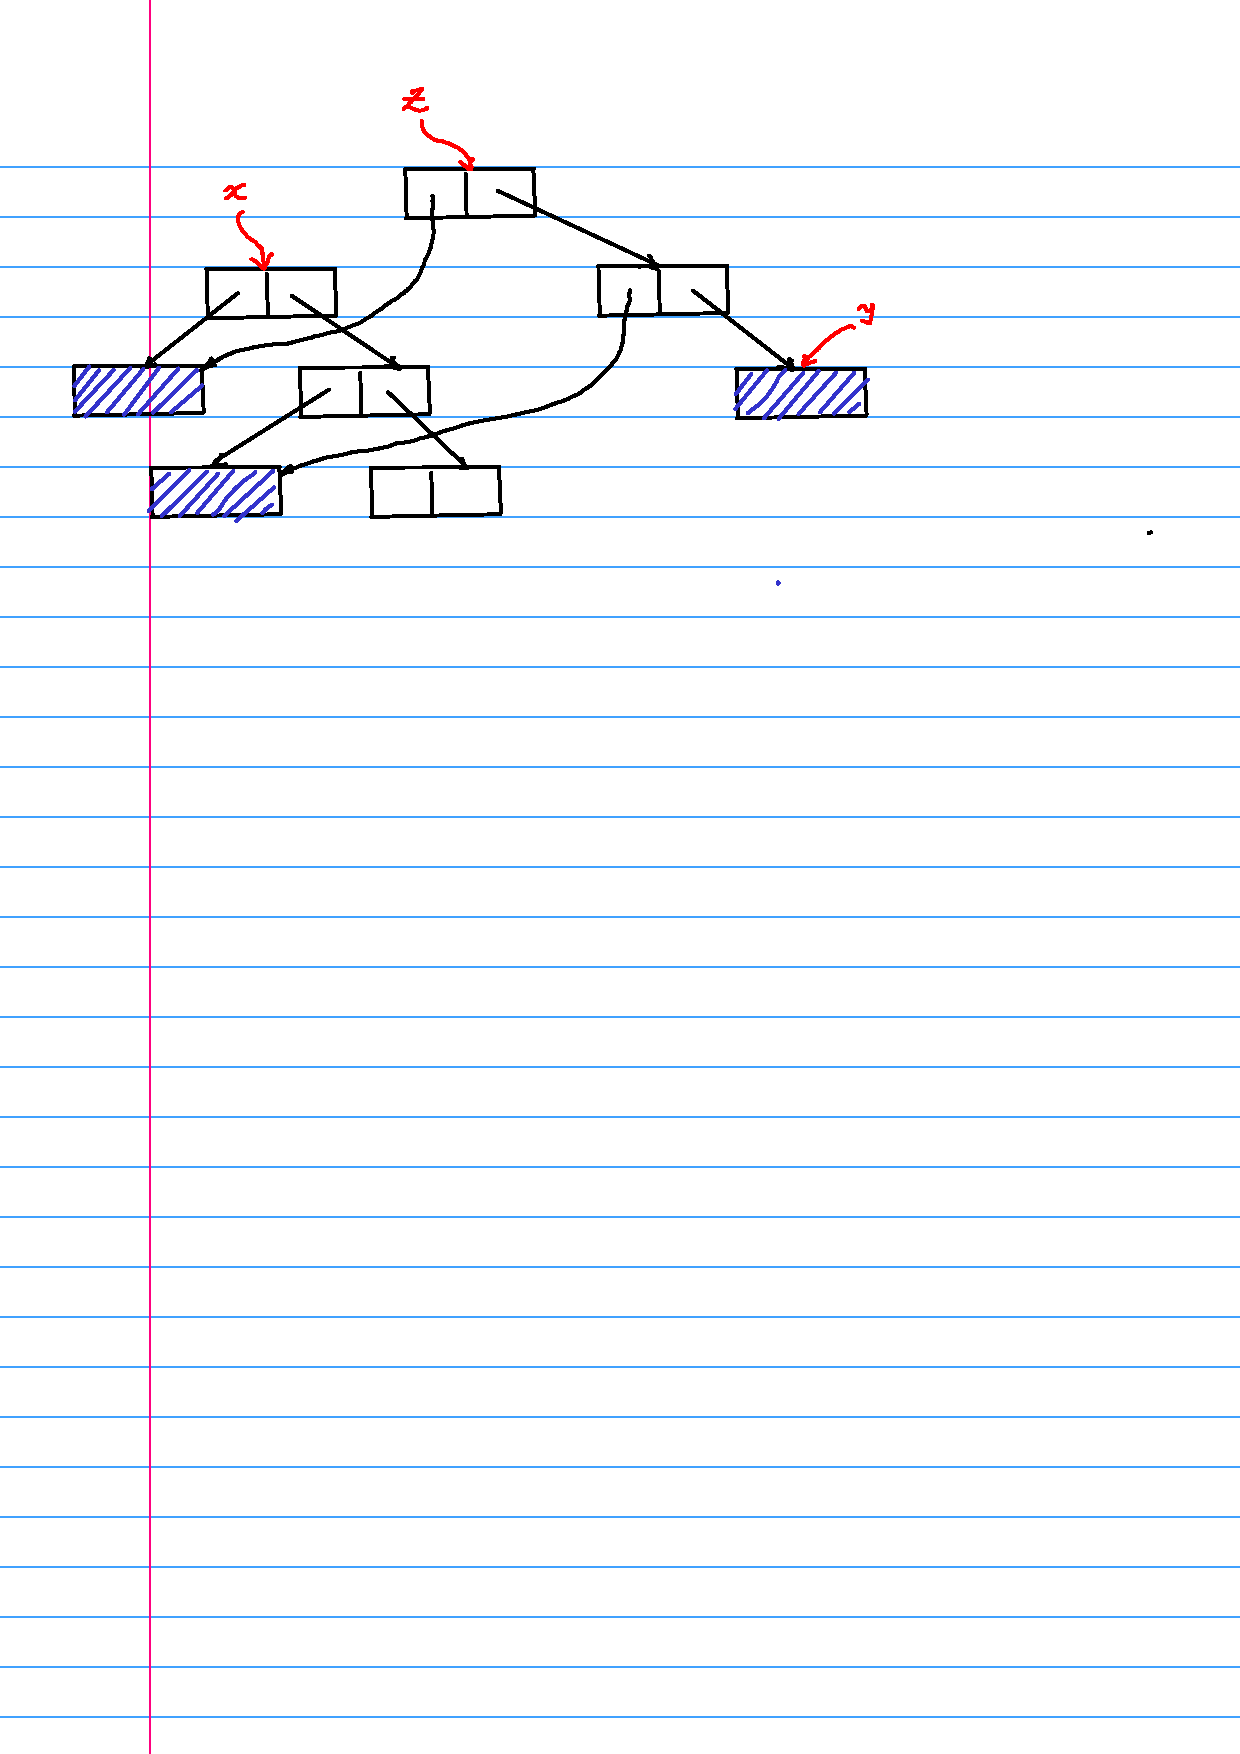
\includegraphics[width=.45\textwidth]{motiv-example}
      %%%%%%%%%%%%%%%%%%%%%Uday's stuff%%%%%%%%%%%%%%%%%%%%%%%%%
\psset{xunit=1mm, yunit=.8mm}
\psset{linewidth=.3mm}
\begin{pspicture}(0,17)(70,57)
%  \psframe(0,17)(70,57)
  %%%%%%%%%%%%%%%%%%%%%%%%%%%%%%%%%%%%%%%%%%%%%%%%%%%%%%%%%%%%%%%%
  \putnode{o}{origin}{13}{40}{\TwoCells{o1}{o2}}
  \putnode{a}{o}{-10}{-15}{\psframebox{5}}
  \ncline[offsetB=-.5,nodesepB=.1]{*->}{o1}{a}
  \putnode{y}{o}{-10}{10}{\psframebox[linestyle=none,framesep=.5]{$\px$}}
  \nccurve[nodesepB=-.2,angleA=330,angleB=120]{->}{y}{o}
  \aput[-2.5](.4){\scalebox{1.2}{\psframebox[framesep=.2,linestyle=none,fillstyle=solid,
	fillcolor=white]{$\times$}}}
  %%%%%%%%%%%%%%%%%%%%%%%%%%%%%%%%%%%%%%%%%%%%%%%%%%%%%%
  \putnode{c}{o}{25}{4}{\TwoCells{c1}{c2}}
  \putnode{d}{c}{10}{-10}{\TwoCellsAD{d1}{d2}}
  \putnode{e}{o}{10}{-15}{\TwoCellsAD{e1}{e2}}
  \putnode{f}{d}{13}{-12}{\TwoCellsAD{f1}{f2}}
  \ncline[nodesepB=-.5]{*->}{c2}{d}
  \ncline[nodesepB=-.5,linewidth=.7]{->}{c2}{d}
  \nccurve[ncurv=1,angleA=235,angleB=45]{*->}{c1}{a}
  \aput[-3.5](.2){\scalebox{1.2}{\psframebox[framesep=.2,linestyle=none,fillstyle=solid,
	fillcolor=white]{$\times$}}}
%  \putnode{g}{e}{-6}{-13}{\TwoCellsAD{g1}{g2}}
  \nccurve[nodesepB=-.5,angleA=240,angleB=30]{*->}{d1}{e}
  \aput[-2.5](.5){\scalebox{1.2}{\psframebox[framesep=.2,linestyle=none,fillstyle=solid,
	fillcolor=white]{$\times$}}}
  \ncline[angleA=300,angleB=110]{*->}{d2}{f}
  \ncline[angleA=300,angleB=110,linewidth=.7]{->}{d2}{f}
  \putnode{w}{c}{-8}{11}{\psframebox[linestyle=none,framesep=.2]{$\pz$}}
  \putnode{ww}{c}{30}{-5}{\psframebox[linestyle=none,framesep=.2]{$\py$}}
  \nccurve[nodesepB=-.2,angleA=330,angleB=120,linewidth=.7]{->}{w}{c}
  %%%%%%%%%%%%%%%%%%%%%%%%%%%%%%%%%%%%%%%%%%%%%%%%%%%%%%%%%%%%%%%%%%
  \ncline[offsetB=-.5,nodesepB=.1]{*->}{o2}{e}
  %\ncline[offsetB=-.1,nodesepB=-.2]{*->}{e1}{g}
  \nccurve[nodesepB=-.3,angleA=270,angleB=90,offsetB=.5]{->}{ww}{f}
  \aput[-3.5](.5){\scalebox{1.2}{\psframebox[framesep=.2,linestyle=none,
        fillstyle=solid, fillcolor=white]{$\times$}}}
  %%%%%%%%%%%%%%%%%%%%%%%%%%%%%%%%%%%%%%%%%%%%%%%%%%%%%%%%%%%%%%%%%%
\end{pspicture}
 \\ 
      \renewcommand{\arraystretch}{.9}
      \begin{tabular}[t]{p{0.9\columnwidth}}
        (b) Memory graph at $\pi$.  \scalebox{.7}{\TwoCellsAD{a1}{a2}}
        denotes a closure. Thick edges denote live links. Traversal
        stops at edges marked $\times$ during garbage collection for
        an ideal collector.
      \end{tabular}
    \end{tabular} 
  \end{pspicture}
  \vspace*{-3ex}
  \caption{Example Program and its Memory Graph}\label{fig:mot-example}
\end{figure}

Figure~\ref{fig:mot-example} shows an example program and the state of
the heap at  the program point $\pi$, i.e. just  before the evaluation
of $(\length\  \pz)$.  The heap is  represented by a graph  in which a
node either  represents atomic  values ($\NIL$,  integers etc.),  or a
\CONS\ cell containing $\CAR$ and $\CDR$  fields, or a chunk of memory
representing  an  unevaluated  value   also  called  a  {\em  closure}
(represented  by  hatched  boxes).   Edges   in  the  graph  are  {\em
  references} and emanate from variables  or fields.  The figure shows
the  lists \px\  and  \pz\ partially  evaluated.   The evaluation  was
triggered    by   the    test   (\NULLQ~(\CAR~(\CDR~\pz)))    in   the
\SIF\ expression.


The edges  shown by thick  arrows are those  which are live  at $\pi$.
Ideally, a cell should be  preserved during garbage collection only if
it is reachable from  the root set through a path  of live edges.  All
other  cells can  be reclaimed.   Thus if  a garbage  collection takes
place at $\pi$ with the heap shown in Figure~\ref{fig:mot-example}(b),
an ideal liveness-based  collector (LGC) will preserve  only the cells
referenced by  $\pz$, $(\CDR~ \pz)$  and (the cells  constituting) the
closure   referenced   by   $(\CDR~(\CDR~\pz))$.    In   contrast,   a
reachability-based collector (RGC) would have preserved all cells.

{\color {Myblue}Rewrite at the end: The specific contributions of the
paper
  are: The formulation of a  liveness analysis for a lazy language and
  the proof of its correctness, the undecidability of the grammar that
  results from the analysis and  its approximation by DFAs, the design
  of a  garbage collector that can  use the DFAs to  retain live cells
  that  also include  closures, and  empirical results  that  show the
  effectiveness of liveness-based garbage collection.}

\subsection{Organization of the paper}

{\color {Myblue}Rewrite at the end: 
Section~\ref{sec:defs} introduces the syntax and semantics of the
language used to illustrate our
analysis.
% Section~\ref{sec:operational} describes the operational semantics of
% the language.
Liveness analysis for this language is  described in
Section~\ref{sec:liveness}. This section also has by  a  sketch  of  a
correctness proof  relative  to  a  non-standard
semantics.  Section~\ref{sec:computing}  shows how to  encode liveness
as   finite-state  automata.    Section~\ref{sec:experiments}  reports
experimental  results  and Section~\ref{sec:lgc-always-better}  proves
that a liveness based collector  can never do more garbage collections
than a reachability based collector.
% and Section~\ref{sec:conclusion} concludes the paper.
}
\section{The target language---syntax and semantics}
\label{sec:defs}
Figure~\ref{fig:lang-syntax} describes the syntax  of our language. It
is a first order language with lazy semantics. Programs are restricted
to        be        in        Administrative        Normal        Form
(ANF)~\cite{chakravarty03perspective} where  all actual  parameters to
functions  are  variables.  While  this  restriction  does not  affect
expressibility,  this form  has  the benefit  of  making explicit  the
creation of  closures through  the $\LET$  construct.  $\LET$s  in our
language  are lazy;  in the  expression $\LET\,\,  x \leftarrow  s\,\,
\IN\,\, e$, $x$ may occur in  $s$. This enables creation of graph-like
structures in  a pure language. The  restriction of \LET\ to  a single
definition  is for  ease  of  exposition---generalization to  multiple
definitions does not add conceptual difficulties.  We further restrict
each variable in a program to  be distinct, so that no scope shadowing
occurs---this  simplifies  the  reasoning   about  the  program.   The
$\SRETURN$  and   \SIF\  expressions  and  strict   operators  trigger
evaluation of closures.

The body  of a function ${\mathit  f}$ is denoted  as $e_{\mathit f}$.
We   shall   extend   this   convention   to   the   main   expression
$e_\mainpgm$. We assume that each program has a distinguished function
\mainpgm\      with      the      definition     $(\DEFINE\      ({\tt
  \mainpgm})\  e_\mainpgm)$ and  the execution  of the  program starts
with the call to \mainpgm.  We write $\pi\!:\!e$ to associate the label
$\pi$ (not  part of the language  syntax) with the  program point just
before expression $e$.

\begin{figure}[t]
\footnotesize
\begin{eqnarray*}
   p \in \mathit{Prog} & \!\!\!::=\!\!\! & d_1 \ldots d_n \,\, e_\mainpgm
    \hspace{5em} \mbox{\em --- program}\\
    \mathit{df} \in Fdef & \!\!\!::=\!\!\! & (\DEFINE\,\, (f\,\, x_1 \,\, \ldots
\,\,x_n)\,\,
    e)
    \hspace{0.2em} \ \ \ \ \mbox{\em --- function definition} \\
e \in \mathit{Expr} & \!\!\!::=\!\!\! &
\left\{\begin{array}{@{}ll@{\hspace{2em}}l}
       (\SIF\,\, x\,\, e_1\,\, e_2) && \!\!\!\mbox{\em --- conditional} \\
       (\LET\,\, x \leftarrow s\,\, \IN\,\, e) &&\!\!\! \mbox{\em --- let
binding} \\
       (\SRETURN\,\, x) && \!\!\!\mbox{\em --- return from function}
    \end{array}\right. \\
s \in \mathit{App} & \!\!\!::=\!\!\!  &
\left\{\begin{array}{@{}l@{\hspace{1.2em}}l}
       k & \mbox{\em --- constant (numeric or $\NIL$)}\\
       (\CONS\,\, x_1\,\, x_2) & \mbox{\em --- constructor} \\
       (\CAR\,\, x) & \\
       (\CDR\,\, x) & \mbox{\em --- selectors} \\
       (\NULLQ\,\, x) & \\
       (\PRIM\,\, x_1\,\, x_2) & \mbox{\em ---  tester
and generic arithmetic} \\
       (\ID\,\, x) & \mbox{\em ---  identity function (for inlining)} \\
       (f\,\, x_1\,\,\ldots\,\, x_n) & \mbox{\em --- function application}
    \end{array}\right.
\end{eqnarray*}
  \caption{The syntax of our language}\label{fig:lang-syntax}
\figrule
\normalsize
\end{figure}


\begin{figure*}[t!]
\begin{center}
\renewcommand{\arraystretch}{1.5}
\begin{tabular}{|c|c|c|}
\hline
Premise & Transition & Rule name \\
\hline
\hline
          & $\rho, (\rho', x, e)\!:\!S, H, \kappa
  \rightsquigarrow \rho', S, H[\rho'(x) := \kappa], e$    &  \sc{const}
\\
\hline
          & {$\rho, (\rho', z, e)\!:\!S, H, (\CONS~x~y)
\rightsquigarrow
$  $\rho', S, H[z := (H(\rho(x)),H(\rho(y)))], e$}     &  \sc{cons} \\
\hline
$H(\rho(x)) \mbox{ is } (d_1, d_2)$ & $\rho, (\rho', z, e)\!:\!S, H,
(\CAR~x)  \rightsquigarrow \rho', S, H[\rho(z) := d_1], e$      &
\sc{car-whnf} \\
\hline
$H(\rho(x)) \mbox{ is } \langle s, \rho'\rangle$ & $\rho, S, H, (\CAR~x)
\rightsquigarrow
\rho', (\rho, x, (\CAR~x))\!:\!S, H, s$      &
\sc{car-clo}
\\
\hline
$H(\rho(x)), H(\rho(y)) \in \mathbb{N}$
 & {$\rho, (\rho', z, e)\!:\!S, H, (+~x~y)  \rightsquigarrow$
$\rho', S, H[\rho(z) \mapsto H(\rho(x)) + H(\rho(y))], e$}      &
\sc{prim-whnf} \\
\hline
$H(\rho(x)) \mbox{ is } \langle s, \rho'\rangle$ & $\rho, S, H, (+~x~y)
\rightsquigarrow
\rho', (\rho, x, (+~x~y))\!:\!S, H, s$      &
\sc{prim-1-clo} \\
\hline
$H(\rho(y)) \mbox{ is } \langle s, \rho'\rangle $ & $\rho, S, H, (+~x~y)
\rightsquigarrow
\rho', (\rho, y, (+~x~y))\!:\!S, H, s$      &
\sc{prim-2-clo} \\
\hline
{$\mathit{f}~\mbox{defined as}$
$~(\DEFINE~(f~\myvec{y})~e_{\mathit{f}})$}  & $\rho, S, H,
(f~\myvec{x})  \rightsquigarrow
[\myvec{y} \mapsto \rho(\myvec{x})], S, H, e_{\mathit{f}}$      &
\sc{funcall} \\
\hline
$\ell$ is a new location& {$\rho, S, H, (\LET~x\leftarrow s~\IN~e)
  \rightsquigarrow$
$\rho\oplus[x \mapsto \ell], S, H[\ell \mapsto \langle s,
    \lfloor\rho\rfloor_{FV(s)}  \oplus [x \mapsto
  \ell]\rangle], e$} &
\sc{let} \\
\hline
$H(\rho(x)) \ne 0$ & $\rho, S, H, (\SIF~x~e_1~e_2)   \rightsquigarrow
\rho, S, H,  e_1$ & \sc{if-true} \\
\hline
$H(\rho(x)) = 0$ & $\rho, S, H, (\SIF~x~e_1~e_2)   \rightsquigarrow
\rho, S, H,  e_2$ & \sc{if-false} \\
\hline
$H(\rho(x)) = \langle s, \rho' \rangle $ & {$\rho, S, H,
  (\SIF~x~e_1~e_2)   \rightsquigarrow
\rho', (\rho, x, (\SIF~x~e_1~e_2))\!:\!S, H,  s$}
&
\sc{if-clo} \\
\hline
{$H(\rho(x))~\mbox{is}$ $\mbox{whnf with value}~v$}& $\rho, (\rho', z,
e)\!:\!S, H,
(\SRETURN~x)  \rightsquigarrow \rho', S, H[\rho(z) \mapsto v], e$ &
\sc{return-whnf}\\
\hline
$H(\rho(x)) = \langle s, \rho' \rangle $ & {$\rho, S, H, (\SRETURN~x)
  \rightsquigarrow$
$\rho',~ (\rho, x, (\SRETURN~x))\!:\!S, H,  s$} &
\sc{return-clo} \\
\hline
\end{tabular}
\caption{A small-step semantics for the language. \label{fig:lang-semantics}}
\end{center}
\end{figure*}



\subsection{Semantics}
We now give  a small-step semantics for our  language.
We first specify the domains used by the semantics:
\[
\begin{array}{@{}r@{\ }l@{\ \ }c@{\ \ }l@{\hspace{0.5em}}l}
\rho: & \mathit{Env} &=&\mathit{Var} \rightarrow \mathit{Loc} & \mbox{-- Environment} \\
v:   & \mathit{Val} &=& \mathbb{N} + \{\NIL\} + \mathit{Data \times Data}& \mbox{-- Values}\\
c:   & \mathit{Clo} &=& \mathit{(Exp \times Env)}& \mbox{-- Closures}\\
d: & \mathit{Data} &=&\mathit{Val} + \mathit{Clo} & \mbox{-- Values \& Closures} \\
\heap: & \mathit{Heap} & =&\mathit{Loc} \rightarrow Data & \mbox{-- Heap}
\end{array}
\]

Here  $\mathit{Loc}$ is  a countable  set  of locations  in the  heap.
Since all data objects are boxed, we model an environment as a mapping
from the set  of variables of the program  $\mathit{Var}$ to locations
in the  heap.  These  either contain  a value in  WHNF (a  number, the
empty  list  $\NIL$,  or  a  \CONS\  cell  with  possibly  unevaluated
constituents) or  a {\em closure}.   A closure  is a pair  $\langle s,
\rho\rangle$ in  which $s$ is  an unevaluated application,  and $\rho$
maps free variables of $s$ to their respective locations.

The  semantics  of   expressions  (and  applications\footnote{In  most
  contexts, we  shall use  the term 'expression' and the notation $e$  for
both  expressions and
  applications.}) are  given by transitions  of the form  $\rho, \stk,
\heap, e \rightarrow \rho', \stk', \heap', e'$.  Here \stk\ is a stack
of  continuation  frames.  Each  continuation  frame  is  of the  form
$(\rho, x, e)$, signifying that the  location of $x$ has to be updated
with the  value of the currently  evaluating expression, and $e$  is to be
evaluated  next  in  the  environment  $\rho$.   The  start  state  is
$([\;]_\rho,([\;]_\rho,  \ans,   (\print~\ans)):[\;]_{S}  ,  [\;]_{H},
(\mainpgm)$.  In  this, the initial  environment and the  initial heap
are  denoted  by  $[\;]_\rho$  and  $[\;]_H$, and  the  initial  stack
consists  of  a  single  continuation   frame  in  which  \ans\  is  a
distinguished  variable  that  would  be  updated with  the  value  of
(\mainpgm).  In  addition, \print\ is a function  modelling a printing
mechanism---a standard  runtime support assumption  for lazy languages
that prints the  value of (\mainpgm).  Notice the  use of the operator
$:$ for adding elements to the top of the stack.




%% In absence of a static type-checking mechanism, programs with other
%% than syntactic  errors lead to states  not covered by  any rules in
%% the small-step semantics.
The notation  $[\myvec{x}   \mapsto  \myvec{\ell}]$   represents  an
environment that maps variables $x_i$
%$x_1,  \ldots, x_n$
to locations $\ell_i$
%$\ell_1,  \ldots,  \ell_n$,
and  $\heap[\ell :=  d]$
indicates the  updation of  a heap \heap\  at $\ell$ with  $d$.  $\rho
\oplus \rho'$  represents the  environment $\rho$ shadowed  by $\rho'$
and $\lfloor \rho \rfloor_X$  represents the environment restricted to
the locations in $X$. Finally $FV(s)$ represents the free variables in
the application $s$.

The small-step semantics  is shown in Figure~\ref{fig:lang-semantics}.
As  a sample,  consider  the  rules  for  $(+~x~y)$, an  application
involving a binary operator strict in both arguments.   When
both $x$  and $y$ are already  in WHNF ({\sc prim-whnf}),  the heap is
updated with the  sum of the arguments and  the next expression to be
evaluated is picked from the continuation on the stack. If either of the
arguments is not in
WHNF  ({\sc  prim-1-clo}  and   {\sc  prim-2-clo}),  it  is  sent  for
evaluation, and a continuation  marks that the evaluation of $(+~x~y)$
has to be resumed after the argument is evaluated.

%==============================================================
\renewcommand{\pp}[2]{\ensuremath{#1\!\!:\!#2}} % prog point



\section{Liveness}\label{sec:liveness}

A variable is {\em live} if there  is a possibility of its value being
used in  future computations and  dead if  it is definitely  not used.
Heap-allocated data needs a richer model of liveness which talks about
liveness of  references.  Using  $\acar$, $\acdr$ to  represent access
using  $\CAR$  and  $\CDR$  fields,  the  liveness  of  the  structure
reachable from a  variable can be represented by a  set of {\em access
  paths}     i.e.     prefix-closed     set     of    strings     from
$\{\acar,\acdr\}^\ast$.  As an example, if $x$ is a list with liveness
$\{\epsilon, \acdr,  \acdr\acar, \acdr\acdr,  \acdr\acdr\acar\}$, then
future computations can only refer up  to the second and third members
of $x$.  A  {\em liveness environment} is a mapping  from variables to
subsets of $\{\acar,\acdr\}^\ast$,  but often expressed as  a set, for
example by writing $\{x.\epsilon, x.\acdr, x.\acdr\acdr, y.\epsilon\}$
instead       of       $[x       \mapsto\{\epsilon,\acdr,\acdr\acdr\},
  y\mapsto\{\epsilon\}, z\mapsto\{\}]$.  In  this notation, $x \mapsto
\{\epsilon\}$ represents access using $x$  itself and $x \mapsto \{\}$
indicates that $x$  is dead.  We associate  liveness environments with
program points.  The  liveness at $\pi:e$ is the  liveness just before
executing $e$.


A  notion  related  to  liveness  is  {\em  demand}.   While  liveness
represents the future use of variables, a demand represents the future
use of the value of an expression.  The demand on an expression $e$ is
again a  set of  access paths---that subset  of $\{\acar,\acdr\}^\ast$
which the context of $e$ may explore of $e$'s result.  To see the need
for  demands,  consider   the  let  expression  $\pi:(\LET~x\leftarrow
(\CDR~y)~\IN~  \pi':\SRETURN~x)$.  Assume  that  the  context of  this
expression produces  the liveness $[x \mapsto  \lbrace \epsilon, \acar
  \rbrace]$ at $\pi'$.  Due to the \LET\ definition which binds $x$ to
$(\CDR~y)$, the  liveness of $x$ at  $\pi'$ now becomes the  demand on
$(\CDR~y)$.    This,  in   turn,  generates   the  liveness   $\lbrace
y.\epsilon, y.\acdr, y.\acdr\acar \rbrace$ at $\pi$. These are the set
of $y$-rooted  accesses required  to explore $\lbrace  \epsilon, \acar
\rbrace$  paths  of  the  result of  $(\CDR~y)$.  In  strong  liveness
analysis       (dual      of       classical      faint       variable
analysis~\cite{horwitz.faint}),  $y$ and  $z$  are live  at the  entry
$\pi: x:=y+z$, if  and only if $x$  is live at exit of  $\pi$.  In our
terminology, the  liveness $\lbrace  \epsilon\rbrace $  of $x$  at the
exit from $n$ becomes the demand on $y+z$, and this, in turn generates
the liveness $\lbrace y.\epsilon, z.\epsilon  \rbrace$ at the entry of
$n$.

We follow the notations appearing in \cite{asati14lgc}. In particular,
We use $\sigma$  to range over demands, $\alpha$ to  range over access
paths and  $\Lv$ to  range over  liveness environments.   The notation
$\sigma_1\sigma_2$  denotes  the  set $\lbrace  \alpha_1\alpha_2  \mid
\alpha_1 \in \sigma_1, \alpha_2  \in \sigma_2\rbrace$.  Often we shall
abuse notation to  juxtapose an edge label and a  set of access paths:
$\acar\sigma$ is a shorthand for $\lbrace\acar\rbrace\sigma$.

\subsection{Liveness Analysis for lazy languages}
\label{sec:liveness-analysis}

%==============================================================
\begin{figure*}[t]
\begin{eqnarray*}
\mathit{ref\/}(\kappa,\sigma,\Lfonly)
          &=& \{\,\} \mbox{, for $\kappa$ a constant, including
$\NIL$}\\
\mathit{ref\/}((\CONS~x~y),\sigma,\Lfonly)
          &=& \{x.\alpha \mid \acar\alpha \in \sigma\} \cup \{y.\alpha
\mid \acdr\alpha \in \sigma\} \\
\mathit{ref\/}((\CAR~x),\sigma,\Lfonly)
          &=&    \begin{array}{l l}
                    \{x.\epsilon\} \cup \{x.\acar\alpha \mid \alpha \in
\sigma\}, & \mbox{if}~\sigma \ne \emptyset\\
                    \emptyset  & \mbox{otherwise}
                 \end{array} \\
\mathit{ref\/}((\CDR~x),\sigma,\Lfonly)
          &=&    \begin{array}{l l}
                    \{x.\epsilon\} \cup \{x.\acdr\alpha \mid \alpha \in
\sigma\}, & \mbox{if}~\sigma \ne \emptyset\\
                    \emptyset  & \mbox{otherwise}
                 \end{array} \\
\mathit{ref\/}((\PRIM~x~y),\sigma,\Lfonly)
          &=&    \begin{array}{l l}
                    \{x.\epsilon, y.\epsilon\},  & \mbox{if}~\sigma \ne
\emptyset\\
                    \emptyset  & \mbox{otherwise}
                 \end{array} \\
\mathit{ref\/}((\NULLQ~x),\sigma,\Lfonly)
          &=&    \begin{array}{l l}
                    \{x.\epsilon\},  & \mbox{if}~\sigma \ne \emptyset\\
                    \emptyset  & \mbox{otherwise}
                 \end{array} \\
\mathit{ref\/}((f~\myvec{x}),\sigma,\Lfonly)
%          &=& \bigcup_{i=1}^n y_i.\Lf{f}{i}{\sigma}
          &=&  \begin{array}{@{}l}  % to discourage \displaystyle
               \bigcup_{i=1}^n x_i.\Lf{f}{i}{\sigma}
               \end{array}
%          &=& \bigcup \{y_i.\Lf{f}{i}{\sigma} \mid i=1,\ldots, n\}
\\[1ex]
\mathcal{L}((\SRETURN~\psi:x),\sigma,\Lfonly) &=& \lbrack \mathit{\epath}
\mapsto
x.\sigma\rbrack, \mbox{ where $\mathit{\epath}$ is a
  new e-path terminating with $\psi$}\\
\mathcal{L}((\SIF~\psi:x~e_1~e_2),\sigma,\Lfonly) &=&
\begin{array}{l l}
                    \mathcal{L}(e_1,\sigma,\Lfonly) \uplus
        \mathcal{L}(e_2,\sigma,\Lfonly) \uplus
        \lbrack\lbrace \mathit{\epath} \mapsto
\{x.\epsilon\}\rbrace\rbrack,  & \mbox{if}~\sigma \ne \emptyset\\
        \emptyset_{\cal{M}}  & \mbox{otherwise}
                 \end{array} \\
&&\mbox{where $\mathit{\epath}$ is a new e-path
  terminating with $\psi$}\\
\mathcal{L}(\LET~x \leftarrow~s~\IN~e),\sigma,\Lfonly) &=&
        \lambda\mathit{\epath}.\; \Lfonly_f(\Lv(x)) \cup \Lv~~
\mbox{where}~\mathcal{M} =
\mathcal{L}(e,\sigma,\Lfonly),~\Lv =
\mathcal{M}(\epath),~\mbox{and}~f~\mbox{is the new function}\\
&& \makebox[0mm]{\hspace*{7cm}
 $(\DEFINE~(f\,x_1\,x_2\, \ldots \, x_n)~(\SIF\,*~x~s[(f\,x_1\,
           x_2\, \ldots\, x_n)/x]))$,} \\
 \makebox[0mm]{\hspace*{8cm} where
     $x_1\, \ldots\, x_n$ are the variables in $s$}
\end{eqnarray*}
\begin{minipage}{0.85\textwidth}
\infrule[live-define]
        {\mathcal{L}(e_f,\sigma,\Lfonly) =
           \bigcup_{i=1}^n z_i.\Lf{f}{i}{\sigma}
              \mbox{ for each $f$ and $\sigma$}
        }
        { \mathit{df_1} \ldots \mathit{df_k} \len \Lfonly
\\ \makebox[0mm]{where
     $(\DEFINE\ (f\ z_1\ \ldots\ z_n)\ \ e_f)$ is a member of $\mathit{df_1}
\ldots \mathit{df_k}$}}
\end{minipage}
  \caption{Liveness equations and judgement rule}\label{fig:live-judge}
\end{figure*}

Figure~\ref{fig:live-judge}  describes  our  analysis  which  has  two
parts. The function $\mathit{ref}$,  takes  an application $s$ and
a demand $\sigma$, and returns  the incremental liveness generated for the
free  variables   of  $s$  due  to  the   application.   The  function
$\mathcal{L}$  uses   $\mathit{ref}$  to  propagate   liveness  across
expressions.

 Since  in a  lazy language,  an  expression is  not evaluated  unless
 required, the null demand ($\emptyset$) does not generate liveness in
 any  of  the  rules  defining  $\mathit{ref}$  or  $\mathcal{L}$.   A
 non-null  demand of  $\sigma$ on  (\CDR~$x$), is  transformed to  the
 liveness $\{x.\epsilon, x.\acdr\sigma\}$.  In  an opposite sense, the
 demand  of $\acdr\sigma$  on  (\CONS~$y$~$z$) is  transformed to  the
 demand  $\sigma$  on $z$.   Since  \CONS\  does not  dereference  its
 arguments, there  is no $\epsilon$ demand  on $y$ and $z$.  The rules
 for (\PRIM~x~y) and (\NULLQ~x) are similar. Constants do not generate
 any liveness.

For the  case of a  function call we  use a third  parameter $\Lfonly$
that  represents  the  summaries  of all  functions  in  the  program.
$\Lfonly_{\mathit  f}$  (the component  of  $\Lfonly$  for a  specific
function $f$), expresses  how the demand $\sigma$ on a  call to $f$ is
transformed into  the liveness of  its parameters at the  beginning of
the   call.    $\Lfonly$  is   determined   by   the  judgement   form
$\mathit{Prog} \len \Lfonly$ using inference rule ({\sc live-define}).
This  rule  describes the  fixed-point  property  to be  satisfied  by
$\Lfonly$, namely, the demand transformation assumed for each function
in  the  program should  be  the  same  as the  demand  transformation
calculated    from    its    body.      As    we    shall    see    in
Section~\ref{sec:grammar-formulation},  we  convert  the rule  into  a
grammar and  the the language generated  by this grammar is  the least
solution satisfying  the rule. We  prefer the least solution  since it
ensures the safe collection of the greatest amount of garbage.

We next  describe the function $\mathcal{L}$  that propagates liveness
across expressions.  Note that,  unlike eager languages, the syntactic
occurrence  of an expression  in a  program denotes  the point  of
creation of its closure, not necessarily its evaluation.
To see the  consequences of this, consider
Figure~\ref{fig:mot-example2} which shows an analysis  of the body of
a function $\length$ with a demand $\sigma$.  Clearly, this is also the
demand on the return value $z$ giving the liveness at the program point
$\pi_8$ as $\{\pz.\sigma\}$.  The liveness at $\pi_8$ is propagated
backwards as in traditional liveness analysis.

Since   \pz\  is   $(1  +   \py)$,  the   liveness  of   $\sigma$  for
\pz\ translates into a demand  of $\sigma$ on $(1+\py)$, which in turn
generates a  liveness of $\{\py.\epsilon\}$ at  $\pi_7$.  We now make
the following observations:
\begin{enumerate}
\item While the liveness of \py\  should be killed at $\pi_6$ since it
  is  beyond the scope  of the  definition of  \py, we  do not  do so.
  However, this  does not cause any  imprecision in the way  of the GC
  marking more cells as live,  since, during execution, \py\ is yet to
  come  into  existence at  $\pi_6$,  and  its  liveness will  not  be
  consulted by the garbage collector at this point.
\item In an  eager language, the heap location referred  by \py\ would
  not have been live at $\pi_8$,  a program point beyond its last use.
  In  a  lazy  language,   however,  the  definition  $\pz  \leftarrow
  (1+\py)$, does not  result in an evaluation of  $(1+\py)$; instead a
  closure  is  created.  The  evaluation  actually  takes place  while
  evaluating $(\SRETURN~\pz)$.   We therefore  record the  liveness of
  $\py$ at  the program point  $\pi_8$, indeed at every  program point
  from $\pi_8$ up to the beginning of the program $\pi_1$ (since we do
  not kill liveness).
\end{enumerate}



We thus  regard the  body of  the function as  an expression  tree and
consider paths from  the root of this tree to  the nodes corresponding
to the program points which trigger evaluation\footnote{Program points
  which      trigger      evaluation       are      labelled      with
  $\psi$.}---\SIF\ conditions and \SRETURN\ expressions.  We call such
paths {\em e-paths}.  For example, for the function \length, there are
three  such paths  $\epath_1 =  \langle \pi_1,  \pi_2, \psi_1\rangle$,
$\epath_2  = \langle\pi_1,  \pi_2,  \pi_3,  \pi_4, \psi_2\rangle$  and
$\epath_3  =  \langle  \pi_1,   \pi_2,  \pi_5,  \pi_6,  \pi_7,  \pi_8,
\psi_3\rangle$.

Given  a function  $\mathit{f}$ and  a demand  $\sigma$,  the liveness
analysis  computes  two   maps:  $\mathcal{L}(e_f,  \sigma,  \Lfonly)$
computes a  map that takes a  e-path in ${\mathit f}$  and returns the
liveness environment  arising out of  all uses of variables  along the
e-path.  A second map $\cal{P}_{\mathit  f}$ maps any program point in
$\mathit f$  to the set  of e-paths sharing  the point.  If  a program
point happens to fall on more  than one such e-path, then the liveness
environment of  the program  point is the  variable-wise union  of the
liveness  environments  of the  individual  e-paths.   In the  example
program,  since ${\mathcal P}_{\length}(\pi_1)  = \lbrace  \epath_1, \epath_2,
\epath_3\rbrace$, the  liveness at $\pi_1$  is ${\cal M}(\epath_1)  \cup {\cal
  M}(\epath_2) \cup  {\cal M}(\epath_3)$,  where ${\cal M}  = \mathcal{L}(e_f,
\sigma, \Lfonly)$.  In the  sequel we shall only define $\mathcal{L}$.
The formulation  of $\cal{P}$ is easy  and we do not  elaborate it any
further.

Consider the  $\mathcal{L}$-rules for {\LET}, {\SIF},  and {\SRETURN}.
The expression  $(\SRETURN~\psi:x)$ with  a demand $\sigma$  forces an
evaluation  of  $x$ and  hence  a  new map  $[\mathit{\epath}  \mapsto
  \{x.\sigma\}]  $ needs  to be  created,  where $\epath$  is a  fresh
evaluation path  terminating in  $\psi$.  The  map for  the expression
$(\SIF~\psi:x~e_1~e_2)$ is a pointwise-union of  the maps of $e_1$ and
$e_2$. In addition, since the condition also triggers an evaluation of
$x$, the map $[\mathit{\epath} \mapsto \{x.\epsilon\}]$ is created and
added  to the  union.  Also  notice a  consequences of  laziness---the
entire  expression including  the condition  is not  evaluated if  the
demand on it is $\emptyset$.  This  results in the empty map, which is
denoted by $\emptyset_{\cal{M}}$.



 The liveness  of {\LET} has  an elegant formulation.   Recollect that
 our language permits lazy {\LET}s whose definitions can be recursive,
 i.e.  in the expression $\LET~x \leftarrow~s~\IN~e$, $x$ can occur in
 $s$.   We  model  the  definition  $x  \leftarrow~s$  as  a  possibly
 recursive function (named $\mathit{f}$ in the rule) which captures an
 arbitrary number of ``unrollings'' of the definition\footnote{The $*$
   in  the definition  of ${\mathit  f}$ represents  non-deterministic
   choice.  During liveness analysis it  can be assumed to generate no
   liveness.}.  We  pass to  the demand  transformer $\Lfonly_{\mathit
   f}$ of this function the demand  arising out of the liveness of $x$
 at the beginning of $e$. This  gives the liveness of the variables of
 $s$.


\mycomment{The function  $\mathcal{L}$ now gives  the (total) liveness
  of  an   expression  $e$.   The  cases  $\SRETURN$   and  $\SIF$  are
  straightforward, but note the liveness $x.\epsilon$ generated by the
  latter.   The case  $(\LET\  z\leftarrow s\  \IN\  e')$ resembles  a
  three-address instruction:  the liveness of  $e$ is given  by taking
  the liveness, $\Lv$, of $e'$, killing any liveness of $z$ and adding
  any incremental  liveness from  $s$.  The main  subtlety is  how the
  liveness of  $z$ in $\Lv$  is converted to  a demand $\Lv(z)$  to be
  placed on $s$ via $\mathit{ref}(s,\Lv(z),\Lfonly)$.


We make three observations: firstly the rule ({\sc live-define}) has a
least  solution  as  $\mathcal{L}(\cdot)$  is monotonic  in  $\sigma$;
secondly  that  ({\sc  live-define})   resembles  the  rule  for  type
inference of mutually recursive  function definitions, and thirdly the
asymmetry of  demand and liveness (compared to  post- and pre-liveness
classically) is due to the functional formulation here.
}

Section~\ref{sec:computing}   shows   how  the   demand   transformers
$\Lfonly$  for  a  program  (representing  a  fully  context-sensitive
analysis) can be safely approximated  by a {\em procedure summary} for
each function.   The summary is  in the  form of a  demand transformer
that maps a demand on a call to the function to demands on each of its
arguments.

\mycomment{\color{red}
\subsection{Correctness of liveness analysis}  
 
We shall now  outline a proof of correctness  of the liveness analysis
presented  in  Section~\ref{sec:liveness-analysis}.   This requires  a
significant modification  to the technique  used in \cite{asati14lgc}.
We shall first modify the standard semantics. This semantics, which we
shall  call {\em  minefield semantics},  will model  a  liveness based
garbage collection at  each transition. This is done  by starting from
the root-set  and inserting a  special value $\bot$ at  each reference
location in the  heap that is reachable but not  live by our analysis.
Attempts  to dereference  such  locations during  the transition  will
result in entering a special  state denoted \bang.  We shall then show
that no program enters the \bang\ state.
 
To set up the minefield semantics, we follow these steps:
\begin{enumerate}
\item  Given an  demand transformer  \Lfonly\ we  enrich  the abstract
  machine state $\rho, S, H, e$  to $\rho, S, H, e, \sigma$.  $\sigma$
  is the  demand on the  currently active function. As  a consequence,
  the liveness $\Lv$ at $e$ is $\mathcal{L}(e, \sigma, \Lfonly)$. Each
  entry  in   the  stack  $S$   of  suspended  evaluations,   is  also
  augmented---it is  now $(\rho, x,  e, eps, \sigma)$. The $\sigma$  in the
  stack entry  represents the demand  on the  function where  the evaluation
  \ldots.  And $eps$ is \ldots.
\item We introduce a function $GC$ that takes the 4-tuple $(\rho, H, S,
  \sigma)$ and  inserts $\bot$ in all locations in the current
  environment $\rho$, the heap $H$ and the environments in the stack
  $S$ that are dead. More formally:





and $\Sigma$ is a  stack of demands---one for each function
  frame pushed in $S$.  Second,  we augment $Val$ with a value $\bot$.
  To model strong liveness $\bot$ may be copied freely, including into
  a  \CONS\  cell,  but  explodes  when  used  computationally  (in  a
  primitive operation  other than a copy). Additionally  we define $GC
  (\Lv, \Sigma)  : (\rho,  H, S) \rightarrow  (\rho ,  H , S  )$ which
  determines live-reachability using $\rho$ and the $\rho$'s in $S$ as
  the root  set and following links in  $H$ only as far  as allowed by
  \Lv\   and   $\Sigma$.     Hence   $GC   (\Lv,   \Sigma)$   replaces
  live-unreachable  values---in $\rho$,  in  $H$ and  the $\rho$'s  in
  $S$---with $\bot$.  For example,  if $x.\epsilon \in \Lv$ then $\rho
  (x) = \bot$.  Only $GC (\cdots )$ introduces $\bot$.
\end{enumerate}  


 }

\section{Computing liveness and its encoding as DFA}\label{sec:computing}
Section~\ref{sec:liveness} gave  a context-sensitive liveness analysis
and  \mycomment{\color  {red}  proved  it  correct  with  reference  to  a  {\em
    minefield} semantics}.  In  particular, $\mathcal{L}$ and \pmap{f}
together described a liveness set for each program point in a function
in terms of  a given $\sigma$ and \Lfonly.  However,  we still have to
describe how to obtain demand transformers \Lfonly\ from the rule {\sc
  live-define} and how to compute the specific demand $\sigma$ on each
function.
%%
To  answer these  questions, it  is convenient  to cast  the equations
arising  out of  $\mathit{ref}$ and  $\mathcal{L}$ as  the rules  of a
grammar.   To do  so, we  need  to modify  the rules  themselves to  a
different form.

\subsection{Modifying liveness rules}

The      $\mathit{ref}$     rule      for     \CONS,      shown     in
Figure~\ref{fig:live-judge},  requires   us  to  remove   the  leading
\acar\ and \acdr\  from the access paths in  $\sigma$.  Similarly, the
rules for  \CAR, \CDR, \PRIM, \NULLQ,  and \SIF\ require  us to return
$\emptyset$, if  $\sigma$ itself is $\emptyset$ and
$\lbrace\epsilon\rbrace$ otherwise.  To  realize these rules
$\sigma$ needs to be known. This creates difficulties since we want to
solve the equations arising out of liveness symbolically.

The  solution  is  to  also   treat  the  operations  mentioned  above
symbolically.  We  introduce three new symbols:  \bcar, \bcdr, \clazy.
These symbols are defined as a relation $\hookrightarrow$ between sets
of access paths:
\begin{align*}
  &\bcar\sigma \hookrightarrow \sigma' \mbox{ where } \sigma' = \{\alpha \mid \acar\alpha \in \sigma\}\\
  &\bcdr\sigma \hookrightarrow \sigma' \mbox{ where } \sigma' = \{\alpha \mid \acdr\alpha \in \sigma\}
\end{align*}
Thus \bcar\ selects those entries in $\sigma$ that have leading \acar, and removes the leading \acar\ from them.
The symbol \clazy\ reduces the set of strings following it to a set containing only $\epsilon$. It filters out, however, the empty set of strings.
\begin{align*}
  \clazy\sigma \hookrightarrow & \left\{ 
  \begin{array}{ll}
    \emptyset&\mbox{if}~\sigma = \emptyset\\
    \{\epsilon\} & \mbox{otherwise}
  \end{array}\right.
\end{align*}
We can  now rewrite the \CONS\  and the \CAR\  rules of $\mathit{ref}$
as:
\begin{align*}
&\mathit{ref\/}((\CONS~x~y),\sigma,\Lfonly)
= x.\bcar\sigma \cup y.\bcdr\sigma  \label{eqn:mod-cons},~
\mbox{and} \\
&\mathit{ref\/}((\CAR~x),\sigma,\Lfonly)
          =   x.\clazy\sigma \cup x.0\sigma
\end{align*}
and the \Lfunonly\ rule
for \SIF\ as:
\begin{align*}
\mathcal{L}((\SIF~x~e_1~e_2),\sigma,\Lfonly) =
                    &\mathcal{L}(e_1,\sigma,\Lfonly)~\uplus
        \mathcal{L}(e_2,\sigma,\Lfonly)~\uplus\\
        &[\,\mathit{\epath} \mapsto  x.\clazy \sigma]
\end{align*}
The rules for  \CDR, \PRIM\ and \NULLQ\ are also  modified in a manner
similar to \CAR. 

When  there  are  multiple  occurences of  \bcar,  \bcdr\  and  \clazy,
$\hookrightarrow$  is  applied  from  right to  left.   The  reflexive
transitive   closure  of   $\hookrightarrow$   will   be  denoted   as
$\stackrel{*}{\hookrightarrow}$.   The  following proposition  relates
the original and the modified liveness rules.
\begin{proposition}
Assume that a liveness computation  based on the original set of rules
gives the liveness  of the variable $x$ at a  program point $\pi_i$ as
$\sigma$   (symbolically,   $\Lanv{i}{x}=   \sigma$).   Further,   let
$\Lanv{i}{x}=  \sigma'$ when the  modified rules  are used  instead of
\Lfunonly.  Then $\sigma' \stackrel{*}{\hookrightarrow} \sigma$.
\end{proposition}

For  an explanation  of why  the  proposition holds  for the  modified
\CONS\  rule,   we  refer   the  reader  to   \cite{asati14lgc}.   The
proposition also holds for other modified rules for similar reasons.

\newcommand{\emm}[2]{\ensuremath{\mathcal{#1}_{#2}}}
\subsection{Generating Liveness Equations}

\begin{figure*}[t!]
  \begin{tabular}{cc}
    \begin{minipage}{.40\textwidth}
        \small
        \renewcommand{\arraystretch}{1}{
          \begin{uprogram}
            \UNL{1} (\DEFINE\ (\length~\xl)
            \UNL{2}  $\pi_1\!\!:\, $(\LET\ \px\ $\leftarrow $\
(\NULLQ~\xl) \IN
            \UNL{3} \hspace*{.05cm} $\pi_2\!\!:\,$(\SIF\
$\psi_1\!\!:\,$ \px
            \UNL{4} \hspace*{.27cm} $\pi_3\!\!:\,
            $(\LET\ \pv\ $\leftarrow 0$ \IN
            \UNL{5} \hspace*{.32cm} $\pi_4\!\!:\,
(\SRETURN~\psi_2:\pv)$
            \UNL{4} \hspace*{.29cm}    $\pi_5\!\!:\, $(\LET~\pu\
$\leftarrow$  (\CDR~\xl)  \IN
            \UNL{5} \hspace*{.34cm}   $\pi_6\!\!:\, $(\LET~\py\
$\leftarrow$  (\length~\pu)  \IN
            \UNL{6} \hspace*{.34cm} $\pi_7\!\!:\,
            $(\LET~\pz\ $\leftarrow$ (1~+~\py) \IN
            \UNL{7} \hspace*{.34cm} $\pi_8\!\!:\,
(\SRETURN~\psi_3:\pz)$)))))))
        \end{uprogram}}
        \renewcommand{\arraystretch}{1}{
	  \begin{uprogram}
	  \UNL{1} $(\DEFINE\ (\main)$
           \UNL{2} \!\!$\pi_9\!\!:\, \cred{(\LET\  \pa\  \leftarrow
(\abigfunction\ \acdr)}$ \IN
          \UNL{3} \!\!$\pi_{10}\!\!:\, \cred{(\LET\  \pb\  \leftarrow
(}$\cred{+}$\cred{\ \pa\ \acdr)}$
\IN
	  \UNL{4}   \hspace*{.05cm}$\pi_{11}\!\!:\,      $ \cred{(\LET\ \pc}\
$\cred{\leftarrow  (\CONS\ \pb\ \NIL)}$ \IN
          \UNL{5}   \hspace*{.15cm}    $\pi_{12}\!\!:\,
          $\cred{(\LET\ \pw}\  $\cred{\leftarrow  (\length\ \pc)}$ \IN
          \UNL{6}  \hspace*{.25cm}  $\pi_{13}\!\!:\,
(\SRETURN~\psi_4:\pw)))))$
\end{uprogram}}
        %%}
    \end{minipage}

    &

    \begin{minipage}{.51\textwidth}

        \small
\begin{eqnarray*}
        \mathcal{L}(e_{\length},\sigma,\Lfonly) &=&
              [\;\epath_1 \mapsto \lbrace \px.\clazy \sigma,
\xl.\clazy\sigma\rbrace ,~\epath_2 \mapsto \lbrace \cred{
\pv.\sigma}  \rbrace,\\
 &&          \;\;  \epath_3 \mapsto \lbrace \pz.\sigma,
                \py.\clazy\sigma,
\pu.\Lf{\length}{\mbox{1}}{\clazy\sigma},\\
&&            \;\;\;\;\;\;\;\;\;\;\;\;\;\;\;\;\;
\xl.\{ \acdr\Lf{\length}{\mbox{1}}{\clazy\sigma} \cup
%%\;\;\;\;\;\;\; \;\;\;\;\;\;\;\;\;\;\;\;\;\;\;\;\\
\cred{\clazy\Lf{\length}{1}{\clazy\sigma}}\}\}
             \rbrack \\
            \cal{P_{\mbox{\tiny \length}}} &=&
                [\;\pi_1 \mapsto \lbrace \epath_1, \epath_2, \epath_3 \rbrace,  \
                 \pi_2 \mapsto \lbrace \epath_1, \epath_2, \epath_3
                  \rbrace, \\
&&\;\;  \pi_3 \mapsto \lbrace \epath_2
                  \rbrace ,  \pi_4 \mapsto \lbrace \epath_2
                  \rbrace, \pi_5 \mapsto \lbrace  \epath_3 \rbrace, \\
 &&  \;\;                        \pi_6 \mapsto \lbrace \epath_3 \rbrace,
\pi_7 \mapsto
                   \lbrace \epath_3\rbrace, \pi_8 \mapsto \lbrace \epath_3
\rbrace~\rbrack\\
              \mathcal{L}(e_{\main},\sigma,\Lfonly) &=&
                [\;
                  \epath_4 \mapsto \lbrace \cred {\pw.\sigma,
                                       \pc.\Lf{\length}{\mbox{1}}{\sigma},}\\
&& \;\;\;\;\;\;\;\;\;\;\;\;\;\;\;\;\;\;
\cred{\pb.\bcar\Lf{\length}{\mbox{1}}{\sigma},}
\cred{\pa.\clazy\bcar\Lf{\length}{\mbox{1}}{\sigma}} \rbrace
                               ] \\
               \cal{P_{\mbox{\tiny \main}}} &=&
                  \lbrack~ \cred{\pi_9 \mapsto \lbrace \epath_4 \rbrace,  \
                    \pi_{10} \mapsto \lbrace \epath_4 \rbrace,  \
                   \pi_{11} \mapsto \lbrace \epath_4 \rbrace,} \\
                   && \;\; \cred{\pi_{12} \mapsto \lbrace \epath_4 \rbrace,
\pi_{13} \mapsto \lbrace \epath_4 \rbrace}~\rbrack
\end{eqnarray*}
    \end{minipage} \\
(a)&
(b)
    %% \end{ tabular}}
  \end{tabular}
%\end{picture}
\kern -3ex
%\vspace{0.5in}
\caption{(a) Example program and (b) its liveness
maps.}\label{fig:mot-example2}
\end{figure*}
%================================================================

Given  a  function  $\mathit{f}$,  we now  describe  how  to  generate
equations  for the  demand  transformation \Lfonly$_\mathit{f}$.   The
program in Figure~\ref{fig:mot-example2} serves  as a running example.
Starting   with    a   symbolic   demand   $\sigma$,    we   determine
\Lfun{e_{\mathit{f}}}{\sigma}{\Lfonly}.   In  particular, we  consider
$\Lanv{1}{x_i}$,  the liveness  of  the $i^{\mbox{\footnotesize  th}}$
parameter   $x_i$  at   the  program   point  at   the  beginning   of
$e_{\mathit{f}}$   (assumed  to   be  $\pi_1$).   By  the   rule  {\sc
  live-define},      this     should      be      the     same      as
$\Lf{f}{i}{\sigma}$. Applying this to \length, we have:
\begin{eqnarray*}
&& \Lanv{1}{\xl} = \clazy\sigma \cup \acdr\Lf{\length}{1}{\clazy\sigma}
  \cup \clazy\Lf{\length}{1}{\clazy\sigma}
\end{eqnarray*}
and  the only equation defining \Lfone{\length} is:
  \begin{eqnarray*}
   && \Lf{\length}{1}{\sigma}
    =  \clazy\sigma \cup \acdr\Lf{\length}{1}{\clazy\sigma} \cup
\clazy\Lf{\length}{1}{\clazy\sigma}
\end{eqnarray*}

In general, the equations for  \Lfonly\ are recursive since, as in the
case  of  \length,  \Lan{1}\  may   have  been  defined  in  terms  of
\Lfone{\mathit{f}}.  However,  it is desirable  to have a  closed form
solution for $\Lfone{\mathit{f}}$.  As mentioned in \cite{asati14lgc},
each  of the liveness  rules modifies  a demand  by prefixing  it with
symbols  in the  alphabet  $\lbrace \acar,  \acdr,\bcar, \bcdr,  \clazy
\rbrace$, and therefore we can assume that $\Lf{f}{i}{\sigma}$ has the
closed form:
\begin{eqnarray}
\label{eq:LF:DI}
  \Lf{f}{i}{\sigma} = \Df{f}{i}\sigma
\end{eqnarray}
where \Df{f}{i} are sets of strings over the alphabet mentioned above.
Substituting   the   guessed   form   in   the   equation   describing
\Lfonly$_{\mathit f}$, and factoring  out $\sigma$, we get an equation
for  \Df{f}{i} that  is  independent of  $\sigma$.   Any solution  for
\Df{f}{i}  yields a  solution for  \Lfonly$_{\mathit f}$.   Applied to
\Lfonly$_{\mathit \length}$, we get:
  \begin{eqnarray*}
&&  \Lf{\length }{1}{\sigma} = \Df{\length}{1}\sigma,~\mbox{and}\\
&&   \Df{\length}{1} = \clazy \cup \acdr\Df{\length}{1}\clazy
       \cup \clazy\Df{\length}{1}{\clazy}
  \end{eqnarray*}

Note that this equation can also be viewed as a CFG with \{\acdr,
\clazy\} as terminal symbols and \Df{\length}{1} as the sole
non-terminal.

\subsection{Generating liveness equations \Lv\  for function bodies}
\label{sec:bodylivenessbodies}

To avoid analyzing the body of a function for each call, we calculated
the liveness  for the arguments and  the variables in  a function with
respect to a symbolic demand  $\sigma$.  To get the actual liveness we
calculate an over-approximation of the  actual demands made by all the
calls and calculate the liveness at each GC
point inside the  function based on this approximation.
The  0-CFA-style  {\em
  summary demand}  is calculated by taking  a union of  the demands at
every call site of a function.

Consider a function $g$ containing a  call to $f$ at a site $\pi$, say
$\pi\!\!:\!(\LET~x   \leftarrow   (f\,y_1\,\ldots\,y_n)~\IN~\pi_i:e)$.
Let the  demand on $g$  be $\sigma_g$ and,  based on this  demand, the
liveness of  $x$ at $\pi_i$ be  $\Lanv{i}{x}$.  By the  $\LET$ rule of
Figure~\ref{fig:live-judge},    the   call   at    $\pi$   contributes
$\Lanv{i}{x}$ to the demand $\sigma_f$. Let us denote the contribution
of a call  site $\pi$ in a  function $g$ to the overall  demand on the
function $f$  as $\deltacall{f}{\pi}{g}$. Assuming that  there are $k$
call sites to function $f$, $\pi^1$ (in function $g^1$) \ldots $\pi^k$
(in   function  $g^k$),  the   over-approximation  of   $\sigma_f$  is
$\deltacall{f}{\pi^1}{g^1}          \cup          \cdots          \cup
\deltacall{f}{\pi^k}{g^k}$.  The distinguished function \mainpgm\ is a
special case.   We assume  it is called  through a  printing mechanism
with   demand   $\sigma_\mainpgm   =  \{\acar,\acdr\}^\ast$ (denoted
$\sigma_{\!all}$) if \mainpgm\ returns a structure and $\epsilon$ if
it returns a base value.


For  the  running  example,   $\length$  has  calls  from  $\main$  at
$\pi_{12}$ and a recursive call at $\pi_6$.
So $\sigma_{\length} =
     \deltacall{\length}{\pi_{12}}{\main}  \cup
\deltacall{\length}{\pi_6}{\length}$.
Filling in  the values gives:
\begin{eqnarray*}
\sigma_{\length}    &=&
 \{\epsilon\}  ~\cup~{\clazy\sigma_{\mathit{\length}}}
\end{eqnarray*}
As examples, the liveness of \Lanv{1}{\pl} and \Lanv{9}{\pa} in terms
of  $\sigma_{\length}$ are:
\begin{align*}
\Lanv{1}{\pl} &= (\clazy \cup \acdr\Df{\length}{1}\clazy
  \cup \clazy\Df{\length}{1}{\clazy})\sigma_{\mathit{\length}}
 \\
\Lanv{9}{\pa} &= \clazy \bcar \Df{\length}{1}\{\epsilon\}
\end{align*}

In summary, the equations generated during liveness analysis are:
\begin{enumerate}
\item For each function $\mathit{f}$, equations defining \Df{f}{i} for
  use by \Lfonly$_{\mathit f}$.
\item For each function $\mathit{f}$, an equation defining the summary
  demand $\sigma_{\mathit f}$ on $e_f$.
\item  For  each  function   $\mathit{f}$  (including  $\mainpgm$  for
  $e_\mainpgm$)  an equation  defining liveness  at each  GC point  of
  $e_{\mathit f}$.
\end{enumerate}
\subsection{Solving liveness equations---the grammar
interpretation}\label{sec:grammar-formulation}
The  equations above can now be re-interpreted as a
context-free grammar (CFG)  on the alphabet $\lbrace\acar, \acdr,
\bcar, \bcdr, \clazy\rbrace$.  Let  \var{$X$} denote the non-terminal
for
a variable  $X$ occurring on  the LHS of the  equations generated
from the analysis.  We can  think of the resulting productions as
being associated with several  grammars, one for each non-terminal
\var{\Lanv{i}{x}} regarded as a start symbol.  As an example, the
grammar    for   \var{\Lanv{1}{\xl}}   comprises    the   following
productions:
\begin{eqnarray*}
  \var{\Lanv{1}{\xl}}  &\rightarrow& 
  \clazy\var{\sigma_{\length}} \mid \acdr \var{\Df {\length}{1}}{\clazy\var{\sigma_{\length}}}  \\
  & & \mid
  \clazy\var{\Df{\length}{1}}{\clazy\var{\sigma_{\length}}} \\
  \var{\Df{\length}{1}} &\rightarrow& \clazy \mid
  \acdr\var{\Df{\length}{1}}\clazy
       \mid \clazy\var{\Df{\length}{1}}{\clazy}\\
\langle {\sigma_{\length}} \rangle
&\rightarrow&
\epsilon  \mid \clazy\langle{\sigma_{\length}}\rangle \\
\var{\Lanv{9}{\pa}} &\rightarrow& \clazy \bcar \var{\Df{\length}{1}}
\end{eqnarray*}
Other equations can be converted similarly.  The language generated by
\var{\Lanv{i}{x}},  denoted  $\mathscr{L}(\var{\Lanv{i}{x}})$, is  the
desired solution  of \Lanv{i}{x}.  However,  note that the  strings in
the  language are  over alphabet  $\lbrace \acar,  \acdr,\bcar, \bcdr,
\clazy \rbrace$, but  we want {\em forward} access paths  only, i. e.,
access paths over the alphabet $\lbrace \acar, \acdr \rbrace$. In
other words,  the decision  problem that we  are interested  in during
garbage collection at a program point $\pi_i$ is:
\begin{quote}
Let  $x.\alpha$ be  a forward  access  path consisting  only of  edges
\acar\    and   \acdr\    (but    not   \bcar, \bcdr\ or \clazy).     Let
$\mathscr{L}(\var{\Lanv{i}{x}}) \stackrel{*}{\hookrightarrow} \sigma$,
where $\sigma$ consists  of forward paths only. Then  does $\alpha \in
\sigma$?
\end{quote}

We now model the above problem  as one of deciding the membership of a
context-free  grammar  augmented  with  a fixed  set  of  unrestricted
productions.

\begin{definition}\label{def:specialgrammar}
Consider a form of  grammar $(N,T, p_1\cup p_2,S)$ in which $N$ is a set of
non-terminals, $T = \{\acar, \acdr, \bcar, \bcdr, \clazy, \$\}$, $p_1$
is a set of context-free production that contains the distinguished
production $S \rightarrow \alpha\$$, $\alpha$ is a string of grammar
symbols that does not contain $S$, and $p_2$ is the fixed set of
unrestricted productions $\bcar\acar \rightarrow \epsilon$,
$\bcdr\acdr \rightarrow \epsilon$, $\clazy\acar \rightarrow \clazy$,
$\clazy\acdr \rightarrow \clazy$, and $\clazy\$ \rightarrow
\epsilon$.
\end{definition}

From Sections \ref{sec:liveness}  and \ref{sec:computing}, it is clear
that the results of liveness analysis of any program can be modeled by
the kind  of grammar described above. The  following proposition shows
that the converse also holds.
\begin{proposition}
Given    a     grammar    $G$    of    the     form    described    in
Definition~\ref{def:specialgrammar},  it is  possible  to construct  a
program $p$  with program points  $\pi_i$ and variables $x$  such that
the liveness  analysis of $p$  is same as  $G$ except for a  change in
non-terminal names which now have the form \var{\Lanv{i}{x}}.
\end{proposition}
We now show that the decision  problem that is required to be answered
at       garbage      collection       time       is      undecidable.
\newcommand{\state}{\ensuremath{\mathsf{S}}}
\newcommand{\nont}[2]{\ensuremath{\mathsf{S}_{#1}^{#2}}}  
\begin{lemma}
Consider    a    grammar    $G$    of   the    kind    described    in
Definition~\ref{def:specialgrammar} and a forward access path $\alpha$
consisting  of symbols \acar\  and \acdr\  only. The  decision problem
$\alpha \in \mathscr{L}(G)$ is undecidable.
\end{lemma} 
\begin{proof}
Given a  Turing machine  and an input  $w\in (1+0)^*$, we  construct a
grammar $G$  such that  the machine will  halt on  $w$ if and  only if
$\epsilon \in  \mathscr{L}(G)$. The grammar includes the  fixed set of
unrestricted productions  in Definition~\ref{def:specialgrammar}. 

We  shall   denote  the  configuration   of  the  Turing   machine  as
$w_l(\state,c)w_r$, where $w_l$ is the string to the left of the head,
$w_r$ is the string to the right, $c$ is the symbol under the head and
\state\ is the current state  of the machine.  For each combination of
state  and   symbol  $(\state,c)$,   the  grammar  will   contain  the
non-terminal \nont{}{c}. We shall synchronize each move of the machine
to a  derivation step  using a context  free production,  followed, if
possible, by  a derivation step  using either $\bcar\acar    \rightarrow
\epsilon$ or $\bcdr\acdr    \rightarrow
\epsilon$.
After each synchronization, we shall establish the following invariant
relation between the machine configuration and the  sentential form:

\begin{quote}
  If the configuration of the machine is $w_l(\state,c)w_r$, then the
  sentential form will be $\overline{w}_l\nont{}{c}\,w_r$, where
  $\overline{w}_l$ is the same as $w_l$ but with each symbol $d$ in $w_l$
  replaced by $\overline{d}$.
\end{quote}

Assume that  the TM starts  in a  state $S_\mathit{init}$ with  a tape
$cw$ and  the head positioned on  the symbol $c$. Then  the sentential
form    corresponding     to    the    initial     configuration    is
$\nont{\mathit{init}}{c}w$ (we  can assume that there  is a production
$\nont{}{} \rightarrow  \nont{\mathit{init}}{c}w$, where  \nont{}{} is
the start symbol of the  grammar). Further correspondences between the
Turing machine moves and the grammar productions are as follows:

\begin{enumerate}
\item For each transition  $(S_i, c) \rightarrow (S_j,c',L)$, there are
  two  productions $\nont{i}{c}  \rightarrow  \acar \nont{j}{\acar}c'$
  and $\nont{i}{c} \rightarrow \acdr \nont{j}{\acdr}c'$.
\item For each  transition $(S_i, c) \rightarrow (S_j,c',R)$, there
  are two productions
  $\nont{i}{c} \rightarrow c \nont{j}{\acar}\bcar$ and $\nont{i}{c}
  \rightarrow c \nont{j}{\acdr}\bcdr$. 
\end{enumerate}
The idea behind  the productions is explained with  an example: Assume
that        the        current        sentential        form        is
\bcar\bcdr\nont{i}{\acar}\acar\acar.  Assume that  the  machine has  a
transition  $(S_i,\acar) \rightarrow (S_j,\acdr,  L)$. Since  the next
corresponding step in the derivation  has to be done without any prior
knowledge of whether the symbol to the left of the tape is a \acar\ or
a  \acdr, two  productions are  provided,  and the  invariant will  be
maintained  only   if  the  production   $\nont{i}{\acar}  \rightarrow
\acdr\nont{j}{\acdr}\acdr$  is  chosen  for   the  next  step  in  the
derivation.         This         gives        the        configuration
\bcar\bcdr\acdr\nont{i}{\acdr}\acdr\acar\acar.    Simplification  with
the    production    $\bcdr\acdr    \rightarrow    \epsilon$    yields
\bcar\nont{i}{\acdr}\acdr\acar\acar, which  exactly corresponds to the
changed configuration  of the machine.  Notice carefully that  a wrong
choice breaks the invariant and it cannot be recovered subsequently by
any choice of productions.

After  the Turing machine  has halted,  there are  further ``cleanup''
derivations  that derive  $\epsilon$ only  if the  invariant  has been
maintained  so far.  For every  symbol  $c$, we introduce  a  non-terminal
$\nont{\mathit{final}}{c}$ where $\nont{\mathit{final}}{}$ is the
final state of the Turing machine. We add
productions $\nont{\mathit{final}}{c} \rightarrow \acar
\nont{\mathit{final}}{c}$ and $\nont{\mathit{final}}{c} \rightarrow \acdr
\nont{\mathit{final}}{c}$ for cleaning up the \bcar\ and \bcdr\ symbols on
the left of the head and $\nont{\mathit{final}}{c} \rightarrow 
\nont{\mathit{final}}{c}\bcar$ and $\nont{\mathit{final}}{c} \rightarrow 
\nont{\mathit{final}}{c}\bcdr$ for cleaning up \acar\ and \acdr\ on the
right of the tape head. This completes the reduction.
\end{proof}

We circumvent the problem  of undecidability by over- approximating the
CFG by non-deterministic finite state automata (NFA). The NFA are then
simplified using  the $\hookrightarrow$ rules.  Finally the simplified
NFAs are converted to DFAs.

%------------------------------------------------------------%
\subsubsection{From CFGs to GC-ready DFAs}
\label{sec:NFA-approx}
 We use  the algorithm by Mohri  and Nederhof~\cite{mohri00regular} to
 approximate a CFG to a {\em strongly regular\/} grammar.  For
 example, the grammar
 fragment  for  the  non-terminal  $\var{\Df{\length}{1}}$  after  the
 Mohri-Nederhof transformation is:
 \begin{eqnarray*}
   \var{\Df{\length}{1}} &\rightarrow& \clazy\var{\Df{\length}{1'}} \mid
   \acdr\var{\Df{\length}{1}}
   \mid \clazy\var{\Df{\length}{1}}\\
   \var{\Df{\length}{1'}} &\rightarrow& \clazy\var{\Df{\length}{1'}}
   \mid \epsilon
 \end{eqnarray*}

The strongly regular grammar is converted  into a set of NFAs, one for
each $\var{\Lanv{i}{x}}$.  The $\hookrightarrow$ simplification is now
done on the NFAs by  repeatedly introducing $\epsilon$ edges to bypass
pairs  of consecutive  edges labelled  \bcar\acar\ or  \bcdr\acdr\ and
constructing the $\epsilon$-closure. Since the $\epsilon$-closure step
may  create  more  adjacent  \bcar\acar\ and  \bcdr\acdr\  edges,  the
simplification is continued till a fixed point is reached, after which
the edges labelled \bcar \ and  \bcdr are deleted.  The details of the
algorithm, its correctness and termination proofs are given by Karkare
et.  al.~\cite{karkare07liveness,asati14lgc}.  The resulting automaton
has  edges labelled  with  \acar,  \acdr\ and  \clazy\  only. In  this
automaton, for every edge labelled \clazy, we check if the source node
of the edge has a valid path to  a final final state.  If yes, we mark
the mark  the source node as  final. Finally, we remove  all the edges
labelled  \clazy\  and  convert  the automaton  into  a  deterministic
automaton.    This   effectively  implements   the   $\hookrightarrow$
simplification rules for  \bcar, \bcdr, and \clazy\  to obtain forward
paths. While  checking for liveness  during GC, a  forward access-path
only if it can reach a final state.


\begin{figure}[t!]
  \begin{tabular}{cc}
\psset{unit=1mm,nodesep=0mm,labelsep=0.5mm}
\begin{pspicture}(0,-5)(50,12)
  \putnode{t0}{origin}{5}{0}{\var{\Df{\length}{1}}}
  \putnode{t1}{t0}{15}{0}{\pscirclebox{\mbox{\ \ \ \ }}} \hspace{5mm}
  \putnode{t2}{t1}{15}{0}{\pscirclebox[doubleline=true]{\mbox{\ \ \ \ }}}
  \psset{arrows=->}
  \ncline{t0}{t1}
  \ncline{t1}{t2}
  \putnode{l0}{t1}{7}{2}{\clazy}
  \nccurve[angleA=45, angleB=135, ncurv=4, nodesep=-1]{t1}{t1}
  \putnode{l1}{t1}{0}{8}{\acdr, \clazy}
  \nccurve[angleA=45, angleB=135, ncurv=3, nodesep=-1]{t2}{t2}
  \putnode{l2}{t2}{0}{8}{\clazy}
\end{pspicture}
&
\psset{unit=1mm,nodesep=0mm,labelsep=0.5mm}
\begin{pspicture}(0,-5)(30,12)
  \putnode{t0}{origin}{5}{0}{\var{\Df{\length}{1}}}
  \putnode{t1}{t0}{15}{0}{\pscirclebox[doubleline=true]{\mbox{\ \ \ \ }}}
  \psset{arrows=->}
  \ncline{t0}{t1}
  \nccurve[angleA=45, angleB=135, ncurv=3, nodesep=-1]{t1}{t1}
  \putnode{l1}{t1}{0}{8}{\acdr}
\end{pspicture}
\\
(a) & (b) \\
\psset{unit=1mm,nodesep=0mm,labelsep=0.5mm}
\begin{pspicture}(0,-5)(50,12) %\psframe(0,-5)(40,12)
  \putnode{t0}{origin}{5}{0}{\var{\Lanv{9}{\pa}}}
  \putnode{t1}{t0}{9}{0}{\pscirclebox{\mbox{\ \ \ \ }}} \hspace{5mm}
  \putnode{t2}{t1}{12}{0}{\pscirclebox{\mbox{\ \ \ \ }}}
%  \putnode{t3}{t2}{12}{0}{\pscirclebox[doubleline=true]{\mbox{\ \ \ \ }}}
  \psset{arrows=->}
  \ncline{t0}{t1}
  \ncline{t1}{t2}
  \putnode{l0}{t1}{5}{2}{\clazy}
%  \ncline{t2}{t3}
%  \nccurve[angleA=55, angleB=125, ncurv=3, nodesep=-.8]{t3}{t3}
%  \putnode{l2}{tD1}{0}{10}{\acdr}
 \putnode{tD1}{t2}{12}{0}{\pscirclebox{\mbox{\ \ \ \ }}} \hspace{5mm}
  \putnode{tD2}{tD1}{12}{0}{\pscirclebox[doubleline=true]{\mbox{\ \ \ \ }}}
  \psset{arrows=->}
  \ncline{t2}{tD1}
  \putnode{l1}{t2}{5}{2}{\bcar}
  \ncline{tD1}{tD2}
  \putnode{lD0}{tD1}{5}{2}{\clazy}
  \nccurve[angleA=45, angleB=135, ncurv=4, nodesep=-1]{tD1}{tD1}
  \putnode{lD1}{tD1}{0}{8}{\acdr, \clazy}
  \nccurve[angleA=45, angleB=135, ncurv=3, nodesep=-1]{tD2}{tD2}
  \putnode{lD2}{tD2}{0}{8}{\clazy}
\end{pspicture}
&
\psset{unit=1mm,nodesep=0mm,labelsep=0.5mm}
\begin{pspicture}(0,-5)(20,12) %\psframe(0,-5)(40,12)
  \putnode{t0}{origin}{5}{0}{\var{\Lanv{9}{\pa}}}
  \putnode{t1}{t0}{9}{0}{\pscirclebox{\mbox{\ \ \ \ }}} \hspace{5mm}
  \psset{arrows=->}
  \ncline{t0}{t1}
\end{pspicture}
\\
(c) & (d)  \end{tabular}
\caption{(a) The  grammar rules for \var{\Df{\length}{1}}
  converted into an automaton, and (b) its DFA. The same for \var{\Lanv{9}{\pa}}
  are shown in (c) and (d).}\label{fig:example-automata}
\figrule
\end{figure}

Figure~\ref{fig:example-automata}(a)  shows the  NFA that  is obtained
from the grammar for \var{\Df{\length}{1}}.  The final DFA is shown in
Figure~\ref{fig:example-automata}(b).  This expectedly says that given
a  demand $\epsilon$  on  \length,  the liveness  of  its argument  is
$\acdr^{*}$  (the  spine  of   the  list  is  traversed).   Similarly,
Figure~\ref{fig:example-automata}(c)     shows     the     NFA     for
\var{\Lanv{9}{\pa}}.          The         DFA         shown         in
Figure~\ref{fig:example-automata}(d)  does  not   accept  any  forward
paths.   This  reflects  the  lazy  nature  of  our  language.   Since
\length\ does not  evaluate the member elements of  the argument list,
the  closure for  \pa\ is  never evaluated  and is  reclaimed whenever
liveness based GC is triggered beyond $\pi_9$.


\section{The Garbage Collection Scheme}

Our experimental setup consists of  an interpreter for our language, a
liveness  analyzer, and  a single  generation copying  collector.  The
garbage collector  can be  easily configured to  work on the  basis of
reachability (RGC  mode) or use  the liveness DFAs (LGC  mode).  While
exploring the  activation record of a  function, LGC uses  the DFAs at
the latest program  point traversed in the function's  body.  Thus, if
LGC is invoked  at the program point $\pi$, it  would use the liveness
DFAs  at  $\pi$ itself  for  exploring the  root  set  of the  current
activation record. For  any other activation record in  the stack, say
for a function ${\mathit f}$  calling ${\mathit g}$ in the call-chain,
the evaluation  point in ${\mathit f}$  which resulted in  the call to
${\mathit g}$ would be used.

We shall call  a unit allocatable memory as a {\em  cell}.  A cell can
hold  a  basic  value   ($\mathit{bas}$),  the  constructor  \CONS\  $(\mathit{cons~
arg_1~arg_2}$) or   a closure.  The closure, in  turn, can be  one of
($\mathit{unop~arg_1}$),  ($\mathit{ binop~arg_1~arg_2}$)  and  function  application
($\mathit{app~arg_1~arg_2})$.  Here each $\mathit{ arg_i}$ is a reference to another heap
cell or terminated through the function $\mathit{makenull}$.

While exploring the heap, the GC  may encounter closures. In RGC mode,
the closure  will be explored  as usual  and copied by  traversing the
references corresponding to the arguments. Since our liveness analysis
predicts the  liveness of  data in its  evaluated form  only, closures
present a challenge for LGC. LGC will  need to map the liveness of the
free variables of the closure to  their evaluation point.  This is not
straight  forward as  variables may  escape their  creation scope  and
needs to  be handled in an  approximate way.  We describe this in detail next.


\subsection{A liveness-based garbage collection scheme}
\label{sec:live-clo}
  \SetStartEndCondition{ }{}{}%
  \SetKwProg{Fn}{procedure}{\string:}{}
  \SetKwFunction{Range}{range}%%
  \SetKw{KwTo}{in}\SetKwFor{For}{for}{\string:}{}%
  \SetKwIF{If}{ElseIf}{Else}{if}{:}{elif}{else:}{}%
  \SetKwFor{While}{while}{:}{fintq}%
  \AlgoDontDisplayBlockMarkers\SetAlgoNoEnd\SetAlgoNoLine%
  \SetKwFunction{Lgc}{$lgc$}%
  \SetKwFunction{Copy}{$lgcCopy$}%
  \SetKwFunction{LCopy}{$lgcCopy$}%
  \SetKwFunction{RCopy}{$rgcCopy$}%

\begin{algorithm}[t]
  \Fn{\Lgc{}}
     {
       \For {each reference $\mathit{ref}$ in root set}
            {\Copy($\mathit{ref}$)\;}
            $\mathit{copyReferencesOnPrintStack()}$\;  
     }
     
     \Fn{\Copy{$\mathit{ref}$}}
        {
          \If{$\mathit{ref}$ is found live using dfa}
             {
               $\mathit{newRef} = $  $\mathit{dupHeapCell(ref})$\;
               \If{cellType($\mathit{ref}$) is $cons$}
                  {
                    {
                      $\mathit{newCar}  = $  \Copy($\mathit{ref\!.car})$\;
                      $\mathit{newRef.car}   =  newCar$\;
                    }
                    {
                      $\mathit{newCdr}$ =   \Copy($\mathit{ref.cdr})$\;
                      $\mathit{newRef.cdr}   = \mathit{newCdr}$\;
                    }    
                  }
               \If {cellType($\mathit{ref}$) is closure}
                   {
                     $\mathit{newRef.arg1}$ =  \Copy$\mathit{(cell.arg1)}$\;
                     $\mathit{newRef.arg2}$ =  \Copy$\mathit{(cell.arg2)}$\;
                   }
             }
        }

        \caption{LGC with closure collection based on liveness.\label{algo:lgc-a}}
\end{algorithm}
Algorithm~\ref{algo:lgc-a}   describes    a   liveness-based   garbage
collection scheme.  Starting with the root set, each live reference is
explored  using   $\mathit{  lgcCopy}$.    Copying  \CONS\   cells  is
simple---it  just involves  copying  the cell  itself and  recursively
copying the  \CAR\ and the  \CDR\ fields.   On the other  hand copying
closures  requires  determining  the  liveness  of  its  arguments  at
run-time.

Let   us  consider   determining  the   liveness  of   a  closure   at
runtime. Consider a closure $(app~f~y)$  has a reference from the root
set  variable  $x$.  If $x$  is  live,  then  we  know that  the  cell
$(app~f~y)$ has  to be copied.  To copy  the heap structure  rooted at
$y$, we need the liveness of  $y$ at the program point which triggered
the evaluation of  $(app~f~y)$. However, this is only  possible if the
activation record of the function  which created this closure is still
on the activation stack. This does  not always happen since a function
could pack a closure in a \CONS\ cell and return the \CONS\ cell.

An alternative could be to  carry with each closure, extra information
about the program point which triggered its evaluation.  This gives us
precise liveness  information of the  free variables of a  closure but
involves the overhead of updating the program point information during
execution.  To avoid  this overhead we go for a  safe approximation by
storing the {\em creation point of  the closure} and using it to check
liveness.  This  is safe since the  liveness at the creation  point of
the closure dominates  all possible evaluation points  of the closure,
but it  might be imprecise  as the actual  liveness might be  way less
than what is found at the creation point.

Note that  when a reachability-based  collector visits a cell  for the
first time,  it is  marked.  Explorations starting  from the  cell are
curtailed if the cell is visited subsequently due to sharing.  Since a
liveness-based collector may reach the  same cell multiple times, each
time with a different automaton state, this curtailment cannot be done
in the case  of LGC. This is an inherent  drawback of a liveness-based
collector.  This  can be mitigated  by maintaining a list  of liveness
automata states  that a  particular heap cell  was traversed  with and
avoid repeated traversals if we reach the cell in one of these states.
However this also involves storage and run-time penalty.

To  avoid  performance  penalty,  we experimented  with  a  mixed-mode
garbage collection scheme  which uses liveness for  evaluated data and
reachability for closures.

\subsection{Liveness-based collector with reachability-based closure
  collection}
\begin{algorithm}[t]
  \Fn{\Lgc{}}
     {
       \For {each reference $\mathit{ref}$ in root set}
            {\LCopy($\mathit{ref}$)\;}
            $\mathit{copyReferencesOnPrintStack()}$\;  
     }
     \Fn{\LCopy{$\mathit{ref}$}}
        {
          \eIf{cellType$(\mathit{ref})$ is $cons$}
              {
                \eIf {$\mathit{ref}$ is found live using dfa and has not been copied using
                  reachability}
                     {
                       $\mathit{newRef}$ =  $\mathit{dupHeapcell(ref})$\; 
                       $\mathit{ newCar}  =$  \LCopy$\mathit{(ref.car)}$\;
                       $\mathit{ newRef.car}   = \mathit{ newCar}$\;
                       $\mathit{ newCdr}  =$  \LCopy$\mathit{(ref.cdr)}$\;
                       $\mathit{ newRef.cdr}   = \mathit{newCdr}$\;
                     }
                     { $\mathit{makenull(ref)}$\;}}
              {
                \If {cellType$\mathit{(ref)}$ is closure and 
                  has not been copied}
                    { 
                      $\mathit{newRef}$  = \RCopy$(\mathit{ref})$\;
                    }
              }
        }
        \caption{LGC with reachability-based closure collection.\label{algo:lgc-b}}
\end{algorithm}
\begin{table*}[ht!]
\caption{Experimental results comparing RGC and LGC}
\label{tab:experimental-results}
\centering
\begin{tabular}{|@{\ }c@{\ }|@{\ }r@{\ }|@{\ }r@{\ }|@{\ }r@{\ }|@{\ }r@{\ }|@{\ }r@{\ }|@{\ }r@{\ }|@{\ }r@{\ }|@{\ }r@{\ }@{\ }|@{\ }@{\ }r@{\ }|@{\ }r@{\ }|@{\ }r@{\ }|@{\ }r@{\ }|@{\ }r@{\ }|}
\hline
  & \multicolumn{2}{@{}c@{}|}{DFA}
  & \multicolumn{2}{@{}c@{}|}{\# Collected} 
  & \multicolumn{2}{@{}c@{}|}{\# Touched}
  & \multicolumn{2}{@{}c@{}|}{} 
  & \multicolumn{2}{@{}c@{}|}{}
  & \multicolumn{2}{@{}c@{}|}{GC time}
  &  \\ \cline{2-3}
  &   \# & Generation
  &   \multicolumn{2}{@{}c@{}|}{cells per GC}
  &   \multicolumn{2}{@{}c@{}|}{cells per GC}
  &   \multicolumn{2}{@{}c@{}|}{\#GCs}
  &   \multicolumn{2}{@{}c@{}|}{Drag Reduction (\%)}
  &   \multicolumn{2}{@{}c@{}|}{(sec)} &Speedup \\
\cline{4-13}
{Program}&States&Time (sec) &RGC&LGC&RGC&LGC&RGC&LGC&\#Cells&Time&RGC&LGC&RGC/LGC \\
\hline
\hline

\verb@lambda@ & 3312 & 14.7 & 7271.7 & 7517.1 & 13194.2 & 95644.2 & 775 & 750 & 25.60 & 0.71 & 0.16 & 0.94 & 0.17
\\ \hline

\verb@nperm@ & 2055 & 1.1 & 4684.4 & 8633.2 & 22744.2 & 18808.5 & 710 & 386 & 87.96 & 102.07 & 0.23 & 0.14 & 1.62
\\ \hline

\verb@treejoin@ & 2332 & 2690.5 & 50284.2 & 72317.5 & 1566250.0 & 1553000.0 & 116 & 81 & 12.60 & 1.29 & 3.80 & 3.78 & 1.00
\\ \hline

\verb@lcss@ & 2340 & 13.3 & 8064.7 & 10103.6 & 14177.9 & 12542.8 & 30 & 24 & 1.99 & 1.10 & 0.01 & 0.01 & 0.83
\\ \hline

\verb@sudoku@ & 5672 & 798.5 & 983.9 & 1048.8 & 3091.0 & 5650.9 & 169 & 159 & 8.45 & -0.98 & 0.01 & 0.02 & 0.32
\\ \hline

\verb@fibheap@ & 2254 & 49.8 & 4610.8 & 4736.6 & 33389.9 & 35890.1 & 1002 & 975 & 1.25 & 1.49 & 1.07 & 5.08 & 0.21
\\ \hline

\verb@nqueens@ & 1229 & 0.5 & 17048.1 & 21993.1 & 5680.9 & 985.9 & 511 & 396 & 38.52 & 36.29 & 0.05 & 0.02 & 2.08
\\ \hline

\verb@knightstour@ & 1742 & 5.1 & 229973.0 & 289223.0 & 450027.0 & 454813.0 & 412 & 328 & 5.99 & 1.38 & 4.40 & 8.77 & 0.50
\\ \hline

\verb@gc_bench@ & 729 & 0.1 & 21080.6 & 204817.0 & 183769.0 & 33.0 & 34 & 4 & 660783.87 & 1738598.92 & 0.11 & 0.00 & 0.00
\\ \hline

\end{tabular}

\end{table*}

  Algorithm~\ref{algo:lgc-b}  describes  a garbage  collection  scheme
  where the liveness automata is  consulted only for \CONS\ cells; and
  assumes everything under a closure  to be live and copies everything
  that is reachable.
 
A consequence of  copying everything under a closure is  that we might
reach  a non-live  cell that  has been  reclaimed earlier  by liveness
based GC.   This can  happen if  a \CONS\  cell having  partially live
sub-structure  is copied  using liveness  during a  collection and  it
subsequently  becomes part  of a  live closure.   During a  subsequent
collection, the collector may try to copy everything under the closure
including the dead  sub-structure of the \CONS\ cell.   To avoid this,
we ensure  that any non-live  references are not carried  across GC's.
We do this by scanning the live  part of the buffer after every GC and
nullifying any  reference which is  not live. This is  correct because
any reference which  is dead during a collection is  guaranteed not be
dereferenced any further by the program.

Another advantage of  this mixed garbage collection scheme  is that it
avoids the problem of multiple  explorations from the same cell.  This
is done by maintaining a flag in  each cell to indicate whether it was
copied using reachability.

\subsection{Garbage collection for references on print stack}
In lazy  languages the evaluation of  closures is driven  by the print
function~\cite{Jones87}.  Printing of  atomic values is
simple  and  does  not  trigger  a garbage  collection.   In  case  of
\CONS\ cells, the \CAR\ is first  printed followed by \CDR.  In a lazy
language, both \CAR\ and \CDR\ could be closures requiring evaluation,
and this  may trigger  a garbage collection.   When this  happens.  we
have to consider  any references that might be on  the print stack and
copy them. We extend the liveness analysis to the print function and
use its result during garbage collection.

%% Liveness automata  does not exist for  the print function  as it is
%% not part of the executing  program.  Since the print function makes
%% everything  reachable  from a  cell  live  we  can copy  all  cells
%% reachable from the reference.


%% Consider  the case  where a  \CONS\ cells  is being  printed  and a
%% garbage collection  is triggered when  printing the \CDR\  part. In
%% this case, since  the refernce to the \CONS\ cells  is still on the
%% print stack both the \CAR\ and the \CDR\ parts are reachable but we
%% know that the \CAR\ part has already been printed and can be safely
%% garbage collected. A liveness  analysis of the print function would
%% have given  the same information.   In our implementation  we mimic
%% the  behavior of the  liveness analysis  by using  a flag  in every
%% \CONS\ cell which  says whether the \CAR\ part  has been printed or
%% not. For any \CONS\ cell if  the \CAR\ part has not been printed, a
%% reference  to the  \CAR\ part  will also  be on  the stack  but the
%% \CDR\ part has to be explicitly copied.  In case the \CAR\ part has
%% been printed,  then a reference  to the \CDR\  part will be  on the
%% stack and  since the \CAR\ part  is not required anymore  we do not
%% copy anything.  This  optimization subsumes tail call optimization.
%% Again, experimental results show that this optimization minimizes a
%% lot of copying.  \cred{Very sketchy: Make another attempt to write}
%% \hrule

%% \comment{ Unlike  eager languages where  GC happens only  at \CONS~
%%   points or at function calls,  every \LET~ point is a potential GC
%%   point.  The number of automata that needs to be stored is reduced
%%   by sharing  automata along all  the program points along  an {\em
%%   E-path}.

%% By the time the program starts executing, the liveness automata are
%% created  and stored  in a  file.  This  is re-used  every  time the
%% program executes.   An important difference in GC  of lazy language
%% compared to an  eager language is the point  of garbage collection.
%% In case  of eager languages  only \CONS~ points and  function calls
%% are the  GC points. In a  lazy language every \LET~  statement is a
%% potential  GC  point. Hence  we  need  to  store liveness  automata
%% corresponding to  every \LET~ statement in the  program. This leads
%% to an  explosion in  the number of  automata. From  our observation
%% that  along  an {\em  E-path}  all  program  points have  the  same
%% liveness, we  can reduce the  number of automata state  required by
%% sharing  the same  automata for  all program  points along  an {\em
%% E-path}.} In the  example program, we only need  to create automata
%% for program  points \ldots, since  they are the only  distinct {\em
%% E-path}s in the program.






\section{Experimental Evaluation}

%% \comment{To demonstrate the effectiveness of liveness-based garbage collection,
%% we  have  built a  prototype  consisting  of  an interpreter  for  our
%% language,  a  liveness  analyzer  and  a copying  collector  that  can
%% optionally use the results of liveness analysis for marking instead of
%% reachability. When the collector uses liveness for marking, we call it
%% a  {\em liveness-based  collector} (LGC),  else we  use the  term {\em
%%   reachability-based  collector}  (RGC).   The  copying  collector  is
%% neither incremental nor generational.  As a consequence, any cell that
%% becomes unreachable or  dead is assuredly collected in  the next round
%% of garbage collection.}

To   test  the   utility  of   our  method   we  have   implemented  a
garbage-collector for a simple scheme-like first order language having
non-strict semantics. It consists of an interpreter, liveness analyzer
and a  garbage-collector that can  optionally use  reachability or
liveness.  Our  benchmark consists  of programs  from nofib~\cite{nofib}  suite and
some external programs manually converted to ANF.

%% \comment{
%% While exploring the activation record of a function, LGC uses the DFAs
%% at  the latest  program  point traversed  in the function's body.
%% Thus, if  LGC
%% is invoked  at the program point   $\pi$,  it would  use  the
%% liveness  DFAs at  $\pi$ itself for exploring the root set of the
%% current activation record. For any other activation record in the
%% stack, say for a function ${\mathit f}$ calling ${\mathit g}$ in the
%% call-chain,
%% the DFAs at the point of call to  ${\mathit g}$ would be used.}

The process of liveness-based garbage collection involves going through 
each activation record on the stack and exploring each variable in the 
current activation record (root set). The liveness of each variable is 
determined using the program point and the variable name. The liveness 
of all variables are stored as DFAs. These DFAs are then encoded as a 
table. A variable is live only if an entry is found in this table.
All cells that are live are copied to the live semi-space. In case of 
\CONS\ cells the \CAR\ and \CDR\ pointers are chased and if they are 
live the copied \CONS\ cell will get the updated addresses of its 
\CAR\ and \CDR\ fields.


%% \comment{
%% Let $\dfa{\pi}{x}$  denote the DFA  for the variable  and program
%% point  pair ($x$,  $\pi$).  We  assume that  there is  a function
%% $\mathsf{initial}(\dfa{\pi}{x})$  returning the initial  state of
%% $\dfa{\pi}{x}$.
%% Considering   a   DFA   as   a   table,
%% $\dfa{\pi}{x}\mathit{(q,sym)}$  returns the  next  state for  the
%% state $q$ and the  symbol $\mathit{sym}$, where $\mathit{sym}$ is
%% \acar\      or     \acdr.       We      shall     also      write
%% $\dfa{\pi}{x}\mathit{(q,sym)\mathsf{?}}$    for    a    predicate
%% indicating  whether there  is a  transition from  $q$ on
%% $\mathit{sym}$.  The LGC action to chase the root variable $x$ at
%% $\pi$ can be described as  follows: If $\mathscr{L}(\dfa{\pi}{x})$ is
%% empty,  then  nothing  needs  to  be  done.   Otherwise  we  call
%% $\mathsf{copy}(\dfa{\pi}{x},\mathsf{initial}(\dfa{\pi}{x}),    x)$
%% in   Figure~\ref{algo:LGC-main-loop}  and  assign   the  returned
%% pointer to $x$.
%% The function $\mathsf{move\_to\_tospace}(x)$  copies the value of
%% $x$  in the  other semi-space  and returns  the new  address.  It
%% hides  details such as  returning the  forwarding pointer  if the
%% value  of $x$  is  already copied,  and  creating the  forwarding
%% pointer otherwise.}

\subsection{Copying closure using liveness vs copying closures using reachability}
To compare the  effect of using reachability to  copy closures instead
of liveness we take a couple  of programs from our benchmark suite and
execute them with both. As shown in \cred{figure-add-figure-here}, the
number of  garbage collections  in both  cases are  same but  the time
taken  varies largely.  Both these  observations can  be explained  as
follows, since we approximate the  liveness of closure to the liveness
at its  creation point, the  liveness we  get is usually  grossly over
approximated.  Using this liveness may not  give too much of a benefit
compared to  reachability as  nearly everything would  be live  at its
point of  creation.  As mentioned  in Section~\ref{sec:live-clo}, using  liveness for
closures  may  entail  multiple  traversals over  the  same  structure
consuming more time.  Therefore we believe that using reachability for
closures is  a sweet spot in  terms of performance for  liveness based
garbage collectors.
%%
%% \comment{
%% The graphs  in Figure~\ref{fig:memory-usage} show the  number of cells
%% in the heap over time for RGC and LGC---here time is measured in terms
%% of the number of cons cells allocated. In addition, they also show the
%% number of  reachable cells and the  number of cells  that are actually
%% live\footnote{This   is  statically   approximated  by   our  liveness
%%   analysis}.  Since  the programs have  different memory requirements,
%% we have tuned the size of heap for each program to ensure a reasonable
%% number of  collections. An invocation  of RGC decreases the  number of
%% cells  in heap  till  it touches  the  curve of  reachable cells.   An
%% invocation of LGC decreases the number  of heap cells to no lower than
%% the curve of live cells.

%% To construct the  reachable and live curves, we  record for every cell
%% its creation time (\CreateTime), its last use time (\UseTime), and the
%% earliest time  when the  cell becomes unreachable  and can  be garbage
%% collected (\CollTime).  For accurate recording of  \CollTime, we force
%% frequent invocations  of a reachability based collector  in a separate
%% run.     A    cell   is    live    at    time   \mbox{\exectime}    if
%% \mbox{$\mbox{\CreateTime}       \leq       \mbox{\exectime}       \leq
%%   \mbox{\UseTime}$}.       If      \mbox{$\mbox{\CreateTime}      \leq
%%   \mbox{\exectime} \leq \mbox{\CollTime}$}, it is reachable.

%% The benchmark programs are drawn from the {\tt no-fib} suite and other
%% sources and have been  manually converted to  ANF.  All  graphs  except
%%  {\tt  fibheap}  show  fewer  garbage
%% collector  invocations for  LGC. The  number  of reachable  cells in
%% {\tt
%%   fibheap} increases  initially, comes  down before the  heap becomes
%% gets
%% full and then  continues to remains low.  This results in  a single
%% garbage
%% collection in both RGC and LGC.  The graphs also show the precision of
%% our liveness analysis.  For  all programs  except  {\tt nperms} and
%% {\tt lambda} (Figure~\ref{fig:memory-usage-lambda}),  LGC
%% manages to collect a good portion of the data that are not live.}
%%


\subsection{Results}
\newcommand{\hgt}{3cm}
\begin{figure*}[p]
\renewcommand{\arraystretch}{.1}
\begin{tabular}{@{}c@{}c@{}}
   \hskip -4mm{\epsfig{file=lambda.eps, height=\hgt}}
   & {\epsfig{file=lambda_win.eps, height=\hgt}}
\\ \hskip -4mm{\epsfig{file=lcss.eps, height=\hgt}}
&  \hskip -4mm{\epsfig{file=lcss_win.eps, height=\hgt}}
\\ \hskip -4mm{\epsfig{file=gc_bench.eps, height=\hgt}}
&  \hskip -4mm{\epsfig{file=gc_bench_win.eps, height=\hgt}}
\\ \hskip -4mm{\epsfig{file=nperm.eps, height=\hgt}}
&  \hskip -4mm{\epsfig{file=nperm_win.eps, height=\hgt}}
\\ \hskip -4mm{\epsfig{file=fibheap.eps, height=\hgt}}
&  \hskip -4mm{\epsfig{file=fibheap_win.eps, height=\hgt}}
\\ \hskip -4mm{\epsfig{file=sudoku.eps, height=\hgt}}
&  \hskip -4mm{\epsfig{file=sudoku_win.eps, height=\hgt}}
\\ \hskip -4mm{\epsfig{file=nqueens.eps, height=\hgt}}
&  \hskip -4mm{\epsfig{file=nqueens_win.eps, height=\hgt}}
\\ \hskip -4mm{\epsfig{file=treejoin.eps, height=\hgt}}
&  \hskip -4mm{\epsfig{file=treejoin_win.eps, height=\hgt}}
\end{tabular}\vskip -10mm
 \caption{Memory usage  snapshot of  programs.  The  blue and  the red
   curves indicate the  number of cons cells in  the active semi-space
   for  LGC and  RGC  respectively.  The  black  curve represents  the
   number of reachable cells and  the grey curve represents the number
   of cells that are actually live  (of which liveness analysis does a
   static approximation).  x-axis is  the time  measured in  number of
   cons-cells allocated (scaled down by  factor $10^5$). y-axis is the
   number of cons-cells (scaled down by factor $10^3$).}
\label{fig:memory-usage} \figrule
\end{figure*}

Table~\ref{tab:experimental-results} shows  that  LGC
improves the  garbage collection time  and efficiency for most  of the
programs.  Even for  programs where the time taken is  more it is very
competitive.  Memory usage  graphs are shown for  select benchmarks in
Figure~\ref{fig:memory-usage}.  As  the number of  garbage collections
tend  to  be  very large  our  graphs  show  only  a window  which  is
representative of the behavior for  that particular benchmark.  In all
the programs we can see that  the curve corresponding to LGC regularly
dips below the RGC curve.

One area  of concern is the  huge gap between the  actual liveness and
the liveness  percieved by  our collector.  In case  of LGC  for eager
languages  the gap  was  very  narrow and  almost  touched the  actual
liveness curve.  In case of  lazy languages, due to using reachability
for copying we  end up copying more  cells. Any data which  is part of
closure irrespective  of whether it is  live or not gets  copied. Thus
many non-live  cells get  copied during garbage  collection increasing
the drag  time.  Our  experiments have  shown that  unless we  use the
exact  execution  point  for  closures, bringing  down  the  number  of
non-live  cells  copied in  closures  cannot  be reduced.   Using  the
approximated liveness (liveness  at the creation point)  does not give
benefits  in terms  of non-live  cells inside  closures as  everything
would be live at the point of creation.

\section{Related Work} 
\cred{Need to rewrite this entire section need to probably mention some of these 
papers at least i found by googling liveness based GC,\\
http://www.cs.hmc.edu/~oneill/papers/Simplifiers-MSPC.pdf\\
http://costa.ls.fi.upm.es/papers/costa/AlbertGGZ12.pdf\\
http://hirzels.com/martin/papers/ecoop01-gc-liveness.pdf\\
}
Previous attempts to  increase  the space
efficiency
of functional programs by additional  reclamation of memory fall in two
broad categories. In the first,  the program itself is instrumented to
manage  reclamation and reallocation  without the  aid of  the garbage
collector.    Such    attempts   include:   sharing    analysis   based
reallocation~\cite{jones89compile},                       deforestation
techniques~\cite{wadler88deforest,gill93ashort,chitil99deforest},
methods  based  on   linear  logic~\cite{hofmann00linear}  and  region
analysis~\cite{tofte98region}.   Closer  to  our approach,  there  are
methods   that  enable   the   garbage  collector   to  collect   more
garbage~\cite{inoue88analysis,lee05static}   by
explicitly  nullifying  pointers  that  are not  live.   However,  the
nullification,  done   at  compile  time,   requires  sharing  (alias)
analysis.  Our  method, in contrast, does not  require sharing because
of the availability of the heap  itself at runtime.  To the best of our
knowledge, this is the first  attempt at liveness-based marking of the
heap during garbage collection.

%% \begin{figure}[t]
%% \centerline{\epsfig{file=lambda.eps, height=4cm, width=7cm}}
%%  \caption{Memory  usage and garbage collection pattern of  {\tt
%% lambda}.}
%% \label{fig:memory-usage-lambda} \figrule
%% \end{figure}

\section{Conclusions and Future Work}
\label{sec:conclusion}
%% We  have  defined  a  notion  of liveness  on  structured  data;  this
%% generalizes classical liveness and strong liveness.  We started with a
%% general fully context-sensitive analysis  which we proved correct with
%% respect to  a minefield semantics  (this models the effect  of garbage
%% collection between every evaluation step).

%% To  avoid scalability  issues (and  to  avoid performing  part of  the
%% liveness computation at run time)  we defined an 0-CFA version of this
%% liveness analysis  in which  demands for function  $f$ at  all calling
%% contexts are conflated into  a single demand $\sigma_f$.  This enabled
%% us to treat the liveness equations symbolically obtaining context-free
%% grammars for liveness at each GC point (calls to user functions and to
%% $\CONS$).  These were then converted to DFAs for run-time consultation
%% by  the garbage collector.  Experiments confirm  the precision  of the
%% analysis.

%% To obtain performance figures we compared a reachability-based garbage
%% collector with a liveness-based  collector.  This showed a decrease in
%% the  number  of  GCs,   more  garbage  collected  per  invocation.   A
%% significant benefit of LGC is  that programs can run in smaller memory
%% when compared to  RGC. This is potentially useful  in situations where
%% memory  is  limited---as with  embedded  systems.  For  a majority  of
%% programs, the garbage collection times were reduced.

%% One issue we  highlighted was that while fewer  nodes were marked (and
%% more garbage collected), sometimes  cons cells could be visited and
%% traversed  multiple times  with different  sets of  liveness  paths to
%% explore.  Further work includes  improvements to the classical copying
%% collector to reduce the cost of this.
{\color{blue}We extended the liveness based garbage collection to lazy
  languages and shown its benefit  for garbage collection in practical
  programs. We  defined context  senstive liveness analysis  that uses
  context independent summaries of functions obtained using a symbolic
  demand. We show  that obtaining precise solution  to these equations
  is undecidable in  our formulation, and hence  we safely approximate
  the result using DFAs. These DFAs are consulted by garbage collector
  to improve to collection.

  Liveness   of   closure   presented  further   challenges   to   our
  implementation.   We compared  different approximate  strategies for
  handling   liveness   of   closures,   and  found   that   a   mixed
  strategy---reachability  based  collection   of  closure  arguments,
  liveness  based  collection  of   everything  else---works  best  in
  practice as it  avoid runtime and space  overheads.  With mixed-mode
  garbage collection scheme,  we were able to collect  more cells than
  reachability based collectors at a reasonable overhead.

  Although we  provide an  implementation for  a liveness  based garbage
  collection scheme for lazy language, we  do not provide a formal proof
  of its correctness.  A formal  proof of correctness would describe how
  closures  are  handled  during  garbage  collection  and  liveness  is
  propogated inside closures. 

  Another interesting exercise is to narrow the gap between the actual
  liveness and  the perceived liveness  of our garbage  collector. Our
  experiments (not  reported here) show  that a significant  number of
  dead cells  get trapped inside closures.   Using strictness analysis
  to eagerly evaluate closures might  release more of these dead cells
  to be  garbage collected.   Since our  garbage collector  can handle
  closures  (suspended evaluations),  another  major  challenge is  to
  extend it to support higher order programs.

  Orthogonally,  we plan  to improve  the efficiency  of the  liveness
  based garbage collector using heuristics  such as limiting the depth
  of  DFAs,   merging  nearly-equivalent   states  and   using  better
  representation  and algorithms  for automata  manipulation. We  also
  need  to   investigate  the  interaction  of   liveness  with  other
  collection schemes, such as incremental and generational collection.
  In short,  we need to  investigate the  ways to make  liveness based
  garbage collection attractive for practical collectors.  }


%Add graphs for memort usage LGC vs RGC
%Add graphs/table showing the GC times and other statistics

%Mention lower peak memory usage.
%Mention faster GC than full LGC and more garbage collected than RGC.
%Pitch it as sweet spot between full LGC and RGC.
%Future work
%Mention full LGC
%Mention k-liveness, use length example to show 1-liveness is not
%sufficient.
%Mention mixed mode GC,
% - doing RGC most of the times and switching to LGC in case RGC fails
%to collect any garbage
% - doing LGC most of the times but regularly checking the reachability
%of the heap and
% switching to RGC if LGC almost equals RGC

\subsection{References}
\bibliography{fun_hra}{}
\bibliographystyle{abbrv}



\mycomment{
\pagebreak
\pagebreak
\section{Appendix}

We shall now  outline a proof of correctness  of the liveness analysis
presented  in  Section~\ref{sec:liveness-analysis}.   This requires  a
significant modification  to the technique  used in \cite{asati14lgc}.
\cblue{Good points to  make in the main text, right  in the small step
  semantics  section: Note  that the  state of  the  transition system
  consists of the current evaluation context, given by $\rho$ and $e$,
  and  the suspended evaluation  contexts recorded  in the  stack $S$.
  The heap $H$  is common to all contexts.}

The idea behind the proof is  as follows: We shall modify the standard
semantics to a semantics  called {\em minefield semantics} that models
a liveness based garbage collection  at each transition.  The state of
the  transition system  is augmented  to carry  enough  information to
calculate the liveness environment  at the current evaluation context,
and  each   of  the   suspended  evaluation  contexts.    Before  each
transition,  we start  from the  root-set and  insert a  special value
$\bot$ at each  location in the heap that contains  a reference and is
reachable but  not live by  our analysis.  Any attempt  to dereference
such locations during the transition will result in entering a special
state denoted \bang.  The main proof is to show that no program enters
the \bang\ state in the minefield semantics.
 
To set up the minefield semantics, we follow these steps:
\begin{enumerate}
\item We enrich  the abstract machine state $\rho,$ $S,$  $ H,$ $e$ to
  $\rho,$ $S,$ $H,$  $e,$ $\sigma,$ $e_f$.  $\sigma$ is  the demand on
  the expression and $e_f$ is the  body of the function.  The body and
  the demand are both needed to calculate the liveness environment for
  expressions.  The evaluation of  an expression may make variables in
  the scope live because of closures that are created outside it.  The
  information  in a  suspended  evaluation context  is also  similarly
  augmented with the demand on it and the function body of which the
  suspended evaluation is a part.  Thus a stacked entry now takes the
  form $(\rho, x, e, \sigma, e_f)$. A modification of the small step
  semantics which carries the extra information is shown in Figure[].
\item Given the current evaluation context $\rho, S, H, e, \sigma,
  e_f$ and $LF$, we can construct a liveness environment as follows:
  \begin{enumerate}
  \item If $e$ is an expression, then:  
  $$ \Lv = \bigcup_{\psi \in \mathcal{P}(e)} \mathcal{M}(\psi),
    \text{where }
  \mathcal{M} = \mathcal{L}(e_f, \sigma, \Lfonly)$$
\item If $e$ is an application, then:  
  $$ \Lv = ref(e, \sigma, \Lfonly)$$
  \end{enumerate}
We can define in the same way the liveness environment for each of the
suspended  evaluation contexts in  $S$  giving  a  stack of  liveness
environments that we shall denote $\mathsf{SL}$.
\item $GC$ models a liveness based garbage collection:
$GC(\rho,$ $ S,$ $ H,$ $ L,$ $ SL) = (\rho', S', H')$ 
  \begin{enumerate}
  \item For each $x \in domain(\rho)$,  $\rho'(x)=\bot$ iff $x.\epsilon
    \notin \Lv$.
\item For each stack entry $(\rho,\_,\_,\_,\_)$ in $S$ with $\Lv'$ as
  the corresponding liveness environment in $\mathsf{SL}$,  and for each $x
  \in domain(\rho)$,  $\rho'(x)=\bot$
  iff $x.\epsilon \notin \Lv'$.
\item For each location $\ell$, $H'(\ell) = \bot$, iff  there is no
  $x$ in either the current environment or one of the stacked
  environments $\rho$ such that for some $\alpha$, $H[x.\alpha] =
  \ell$  and $x.\alpha \in \Lv$, .
  \end{enumerate}
\end{enumerate}

\begin{figure*}[h!]
\begin{center}
\begin{tabular}{|c|c|c|}
\hline
Premise & Transition & Rule name \\ 
\hline
\hline
          &\makecell{ $\rho, (\rho', x, e, \cred{\sigma', e_f'})\!:\!S,
  H, \kappa, \cred{\sigma, e_f}$ \\ $\rightsquigarrow \rho', S, H[\rho'(x) :=
    \kappa], e, \cred{\sigma', e_f'}$ }   &  \sc{const}
\\
\hline
          & \makecell{$\rho, (\rho', z, e, \cred{\sigma',
    e_f'})\!:\!S, H, (\CONS~x~y), \cred{\sigma, e_f}$ \\ $\rightsquigarrow
  \rho', S, H[z := (H(\rho(x)),H(\rho(y)))], e, \cred{\sigma', e_f'}$}     &  \sc{cons} \\
\hline
$H(\rho(x)) \mbox{ is } (d_1, d_2)$ & \makecell{$\rho, (\rho', z, e,
  \cred{\sigma', e_f'} )\!:\!S, H, (\CAR~x), \cred{\sigma, e_f}$ \\ $
  \rightsquigarrow \rho', S, H[\rho(z) := d_1], e, \cred{\sigma', e_f'}$}      &
\sc{car-whnf} \\
\hline
$H(\rho(x)) \mbox{ is } \langle s, \rho'\rangle$ &\makecell{ $\rho, S,
  H, (\CAR~x), \cred{\sigma, e_f}$ \\ $\rightsquigarrow \rho', (\rho, x,
  (\CAR~x), \cred{\sigma, e_f})\!:\!S, H, s, \cred{(\clazy \cup \acar)\sigma , \_ }$}      &
\sc{car-clo}
\\
\hline
$H(\rho(x)), H(\rho(y)) \in \mathbb{N}$
 & \makecell{$\rho, (\rho', z, e, \cred{\sigma', e_f'})\!:\!S, H,
  (+~x~y), \cred{\sigma, e_f}$ \\  $\rightsquigarrow \rho', S, H[\rho(z)
    \mapsto H(\rho(x)) + H(\rho(y))], e, \cred{\sigma', e_f'}$}      &
\sc{prim-whnf} \\
\hline
$H(\rho(x)) \mbox{ is } \langle s, \rho'\rangle$ &\makecell{$\rho, S,
  H, (+~x~y), \cred{\sigma, e_f}$ \\ $\rightsquigarrow \rho', (\rho, x,
  (+~x~y), \cred{\sigma, e_f})\!:\!S, H, s, \cred{\clazy\sigma, \_}$}      &
\sc{prim-1-clo} \\
\hline
$H(\rho(y)) \mbox{ is } \langle s, \rho'\rangle $ & \makecell{$\rho,
  S, H, (+~x~y), \cred{\sigma, e_f}$ \\ $\rightsquigarrow \rho', (\rho, y,
  (+~x~y), \cred{\sigma, e_f})\!:\!S, H, s, \cred{\clazy\sigma, \_ }$}      &
\sc{prim-2-clo} \\
\hline
{$\mathit{g}~\mbox{defined as}$
$~(\DEFINE~(g~\myvec{y})~e_{\mathit{g}})$}  & \makecell{$\rho, S, H,
  (g~\myvec{x}), \cred{\sigma, e_f}$ \\ $\rightsquigarrow [\myvec{y} \mapsto
    \rho(\myvec{x})], S, H, e_{\mathit{g}}, \cred{\sigma, e_g}$}      &
\sc{funcall} \\
\hline
$\ell$ is a new location& \makecell{$\rho, S, H, (\LET~x\leftarrow
  s~\IN~e), \cred{\sigma, e_f}$ \\ $ \rightsquigarrow \rho\oplus[x \mapsto \ell], S, H[\ell \mapsto \langle s, \lfloor\rho\rfloor_{FV(s)}  \oplus [x \mapsto
  \ell]\rangle], e, \cred{\sigma, e_f}$} &
\sc{let} \\
\hline
$H(\rho(x)) \ne 0$ & \makecell{$\rho, S, H, (\pi:\SIF~\psi:x~e_1~e_2),
  \cred{\sigma, e_f}$ \\ $\rightsquigarrow \rho, S, H,  e_1, \cred{\sigma, e_f}$} & \sc{if-true} \\
\hline
$H(\rho(x)) = 0$ & \makecell{$\rho, S, H, (\pi:\SIF~\psi:x~e_1~e_2),
  \cred{\sigma, e_f}$ \\   $\rightsquigarrow
\rho, S, H,  e_2, \cred{\sigma, e_f}$} & \sc{if-false} \\
\hline
$H(\rho(x)) = \langle s, \rho' \rangle $ & \makecell{$\rho, S, H,
  (\pi:\SIF~\psi:x~e_1~e_2), \cred{\sigma, e_f}$ \\ $\rightsquigarrow
\rho', (\rho, x, (\SIF~x~e_1~e_2),  \cred{\sigma, e_f})\!:\!S, H, s,
\cred{\clazy\sigma, e_f}$}
&
\sc{if-clo} \\
\hline
{$H(\rho(x))~\mbox{is}$ $\mbox{whnf with value}~v$}& \makecell{$\rho,
  (\rho', z, e, \cred{\sigma', e_f'})\!:\!S, H, (\SRETURN~x), \cred{\sigma,
  e_f}$ \\ $\rightsquigarrow \rho', S, H[\rho(z) \mapsto v], e,
  \cred{\sigma', e_f'}$} &
\sc{return-whnf}\\
\hline
$H(\rho(x)) = \langle s, \rho' \rangle $ & \makecell{$\rho, S, H,
  (\psi:\SRETURN~x), \cred{\sigma, e_f}$ \\ $
  \rightsquigarrow$
$\rho',~ (\rho, x, (\SRETURN~x), \cred{\sigma, e_f})\!:\!S, H,  s,
  \cred{\sigma, e_f}$} &
\sc{return-clo} \\
\hline
\end{tabular}
\caption{Minefield semantics for the language.\label{fig:minefield-semantics}}
\end{center}
\end{figure*}
 





%% Generated by bibtex from your ~.bib file.  Run latex,
%% then bibtex, then latex twice (to resolve references)
%% to create the ~.bbl file.  Insert that ~.bbl file into
%% the .tex source file and comment out
%% the command \texttt{{\char'134}thebibliography}.
%% % This next section command marks the start of
%% % Appendix B, and does not continue the present hierarchy
%% \section{More Help for the Hardy}
%% The sig-alternate.cls file itself is chock-full of succinct
%% and helpful comments.  If you consider yourself a moderately
%% experienced to expert user of \LaTeX, you may find reading
%% it useful but please remember not to change it.
%% %\balancecolumns % GM June 2007
%% % That's all folks!





%% % {\color{red}
%% %   (Note 3.\ includes $e_\mainpgm$ treated as the body of
%% %   $(\DEFINE\ ({\tt main})\ e_\mainpgm)$.)
%% % }




%% %% =======

%% %------------------------------------------------------------%
%% %\begin{figure}[t]
  \begin{boxedminipage}{\textwidth}
    \begin{center}
      \raggedright  {\bf  Input:}  Demand $\sigma$ \\
      \raggedright  {\bf  Input:}  Demand Transformer LF \\
      %
      \raggedright{\bf Output:} Modified Liveness Environment Map
      \\
      %  
      \raggedright{\bf Steps:}
      \begin{algorithmic}
        \STATE $M \leftarrow process\_liveness(e, \sigma, LF)$
        \STATE $numargs \leftarrow$ number of arguments in $s$
        \STATE $f \leftarrow$ a new function with $\myvec{x}$ as the argument vector
        
        \FORALL{$l$ in label\_set($e$)} 
        \STATE $var \leftarrow let\_var$ 
        \STATE $rexpr \leftarrow let\_expr$
        \IF {$rexpr$ contains $var$}
        \STATE $L_f \leftarrow process\_liveness (\ f, M[l, x],\ LF)$
        \STATE $le \leftarrow \bigcup_{i=1}^{numargs} x_i.LF_{f}^{i}({\sigma})$
        \ELSE
        \STATE  $le \leftarrow  ref (s,\ \sigma,\ LF)$
        \ENDIF
        \STATE $M[l] = M[l] \bigcup le$
        \ENDFOR
        \RETURN $M$
      \end{algorithmic}
    \end{center}
  \end{boxedminipage}
  \caption{Algorithm for transforming demand for a lazy let}\label{algo:transform-lazy-let} \figrule
\end{figure}

\begin{figure}[t]
  \begin{boxedminipage}{\textwidth}
    \begin{center}
      \raggedright  {\bf  Input:}  Program execution stack  $S$ \\
      \raggedright  {\bf  Input:}  Print stack $P$ \\
      %
      \raggedright{\bf Output:} void \\
      %  
      \raggedright{\bf Steps:}
      \begin{algorithmic}
        \FORALL{$funccall$ in $S$} 
        \STATE $pgm\_pt \leftarrow funccall.return\_pt$
        \FORALL{$var$ in $funccall.varstack$} 
        \STATE $var \leftarrow let\_var$ 
        \STATE $rexpr \leftarrow let\_expr$
        \IF {$rexpr$ contains $var$}
        \STATE $L_f \leftarrow process\_liveness (\ f, M[l, x],\ LF)$
        \STATE $le \leftarrow \bigcup_{i=1}^{numargs} x_i.LF_{f}^{i}({\sigma})$
        \ELSE
        \STATE  $le \leftarrow  ref (s,\ \sigma,\ LF)$
        \ENDIF
        \STATE $M[l] = M[l] \bigcup le$
        \ENDFOR
        \ENDFOR
        \RETURN $M$
      \end{algorithmic}
    \end{center}
  \end{boxedminipage}
  \caption{Algorithm for Liveness based GC}\label{algo:lazy-lgc} \figrule
\end{figure}

}
\end{document}
